\documentclass{beamer}
%Use the [handout] option to eliminate pauses
%\documentclass[handout]{beamer}
%\usetheme{Warsaw}
%\usetheme{Boadilla}
%\usetheme{Madrid}
%\usetheme{Montpellier}
\usetheme{CambridgeUS}

\usepackage{graphicx,amsmath,amssymb,color,multirow, animate}
\usepackage{subfigure}

%\colorlet{newred}{red!60!black}
%\usecolortheme[named=red]{structure}
%\setbeamercolor{block}{bg=white}
% \setbeamertemplate{footline}
%        {
%      \leavevmode%
%      \hbox{%
%      \begin{beamercolorbox}[wd=.333333\paperwidth,ht=2.25ex,dp=1ex,center]{author in head/foot}%
%        \usebeamerfont{author in head/foot}\insertshortauthor~~(\insertshortinstitute)
%      \end{beamercolorbox}%
%      \begin{beamercolorbox}[wd=.333333\paperwidth,ht=2.25ex,dp=1ex,center]{title in head/foot}%
%        \usebeamerfont{title in head/foot}\insertshorttitle
%      \end{beamercolorbox}%
%      \begin{beamercolorbox}[wd=.333333\paperwidth,ht=2.25ex,dp=1ex,right]{date in head/foot}%
%        \usebeamerfont{date in head/foot}\insertshortdate{}\hspace*{2em}
%
%    %#turning the next line into a comment, erases the frame numbers
%        %\insertframenumber{} / \inserttotalframenumber\hspace*{2ex} 
%
%      \end{beamercolorbox}}%
%      \vskip0pt%
%    }
%\setbeamertemplate{blocks}{shadow=true}
%\setbeamertemplate{footline}{\hspace*{.5cm}\scriptsize{\insertauthor 
%\hspace*{50pt} \hfill\insertframenumber\hspace*{.5cm}}}

%\beamertemplatesolidbackgroundcolor{yellow!30}
%\setbeamertemplate{navigation symbols}{}

\begin{document}
%--------------------------------------Title--------------------------------------------------
\title[PhD Proposal]{Application of and Metrics for Lineup Protocols in Different Scenarios }
\author[N. Roy Chowdhury]{PhD Proposal \\ by \\Niladri Roy Chowdhury}
\institute[Iowa State]{Program of Study Committee: \\
Dianne Cook, Major Professor \\
Heike Hofmann, Major Professor \\
Petrutza Caragea \\
Arka Ghosh \\
Eric Cooper}
\date[May 9]{May 9, 2012}


\begin{frame}
	\maketitle
\end{frame}

\begin{frame}
	\begin{itemize}
			  \item 2006 Jul: Bachelor's from University of Calcutta, India.
%			  \item thesis on the fecundability and conception wait in Bangladesh.
%		  \end{itemize}		 
%		\item Employment: 1998-2005
%		  \begin{itemize}
%			  \item computer programmer and database administrator.
%			  \item research in graph theory.
%		  \end{itemize}			 
		\item 2008 Jun: Masters from University of Calcutta, India.
		\item 2008 Aug: Joined Iowa State University, IA.
		\item 2010 Jul: Passed Preliminary Written Exam.
		\item 2010 Dec: Joined Graphical Statistics Group.
%		  \begin{itemize}
%			  \item thesis on Tukey's gh family of distribution
%			  \item research assistant for Traveller's Insurance
%		  \end{itemize}	
%		\item Iowa State University: 2007
%		  \begin{itemize}
%			  \item research for Hy-vee and worked as an intern.
%			  \item after passing preliminary written exam joined graphical statistics group.
%		  \end{itemize}
	\end{itemize}		
\end{frame}


%\begin{frame}
% \frametitle{Statistical graphics}
%  
%		  \begin{itemize}
%			  \item A linear model is fitted to the data.
%			  \item $R^2$ = 0.99.
%			  \item Is it a good model or a bad model?
%			  \item Hold on. Show some plots. We want to see.
%		  \end{itemize}		
%\end{frame}



\begin{frame}
  \frametitle{Visual Inference}
		  \begin{itemize}
		  	\item Plotting data has its origin before the development of classical inference problems.
			  \item Statistical graphics have been used for
			     \begin{itemize}
			        \item exploratory data analysis (EDA).
			        \item model checking and diagnostics (MD).
           \end{itemize}				  
			  \item Can we use statistical graphics for inference?
		  \end{itemize}			
\end{frame}


\begin{frame}
\frametitle{Visual Inference}
  \begin{itemize}
    \item Buja et al (2009)
		  \begin{itemize}
			  \item Introduced method to test the significance of findings.
			  \item Demonstrated formal testing of overall model fitting.
		  \end{itemize}
		\item Protocols of Visual Inference.
		  \begin{itemize}
			  \item Rorschach
			  \item Lineup
		  \end{itemize}		
		\item Application of lineup protocols. 
		  \begin{itemize}
			  \item In a Large $p$ Small $n$ setting.
			  \item Has been the focus of this research.
		  \end{itemize}			
  \end{itemize}		  
\end{frame}


%\begin{frame}
%\begin{center} \Large{Validation} \end{center}
%\end{frame}


\begin{frame}
  \frametitle{Test Statistic}
  
	\begin{columns}
	
		\begin{column}{0.4\textwidth}
		  \begin{itemize}
			  \item Function $T(Y)$ that maps data $Y$ to a plot.
			  \item Associated with a specific null hypothesis.
			  \item A good test statistic should display an extreme feature of the data if it exists.
			  \item The test statistic is a plot of the actual data.		
		 \end{itemize}		
		\end{column}
		
		\begin{column}{0.6\textwidth}
			 \begin{center} \scalebox{0.85}{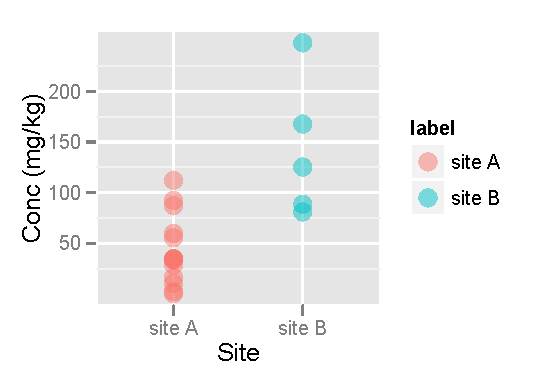
\includegraphics{data-dot.pdf}} \end{center}
		\end{column}
		
	\end{columns} 
	
\end{frame}



\begin{frame}
  \frametitle{Compare Test Statistic with Null Distribution}
	\begin{columns}
		\begin{column}{0.4\textwidth} Lineup plot
		  \begin{itemize}
			  \item A layout of $m=a \times b$ plots.
			  \item One of the plots is of observed data.
			  \item All other plots are generated by a process consistent with the null hypothesis.
			  \item Reject null hypothesis if observed plot is identified.
			  %\item Data from more than one person can be used to assess the significance.
		  \end{itemize}		
			
		\end{column}
		
		\begin{column}{0.6\textwidth}
			 \begin{center} \scalebox{0.5}{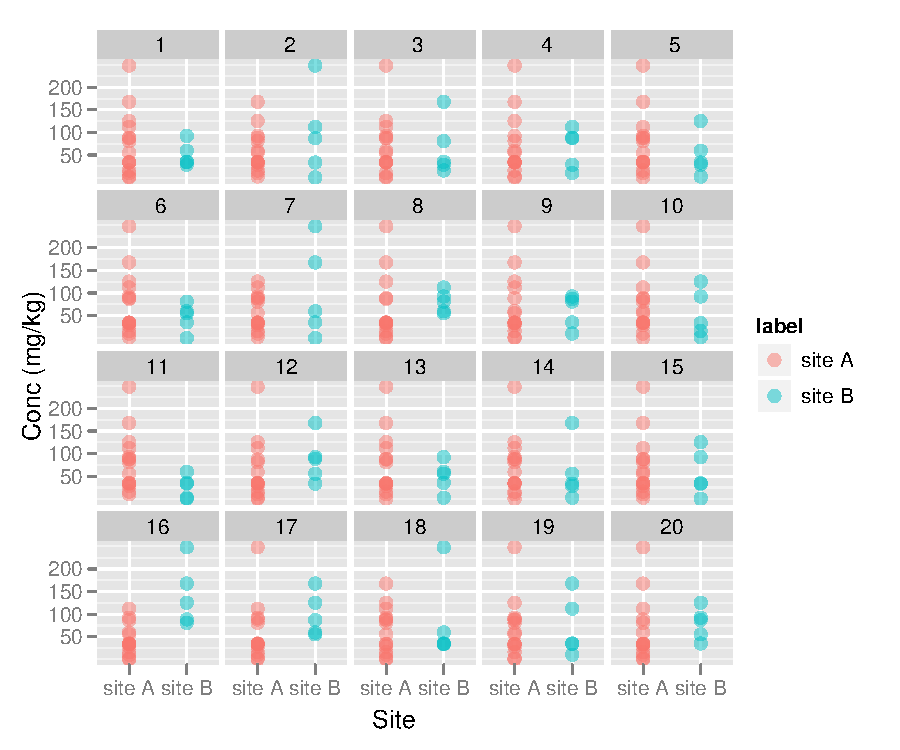
\includegraphics{lineup-dot.pdf}} \end{center}
		\end{column}
	\end{columns}  
\end{frame}

\begin{frame}
  \frametitle{Example}
  
	\begin{columns}
	
		\begin{column}{0.4\textwidth}
		  \begin{itemize}
			  \item To test $H_0: \mu_1 = \mu_2$ vs $H_a: \mu_1 \ne \mu_2.$
			  \item The test statistic is the plot of the real data.
			  \item The null plots are generated by permuting class variable keeping the continuous variable fixed.			
			    \item We reject $H_0$ if the observed plot is identified.		
		 \end{itemize}		
		\end{column}
		
		\begin{column}{0.6\textwidth}
			 \begin{center} \scalebox{0.5}{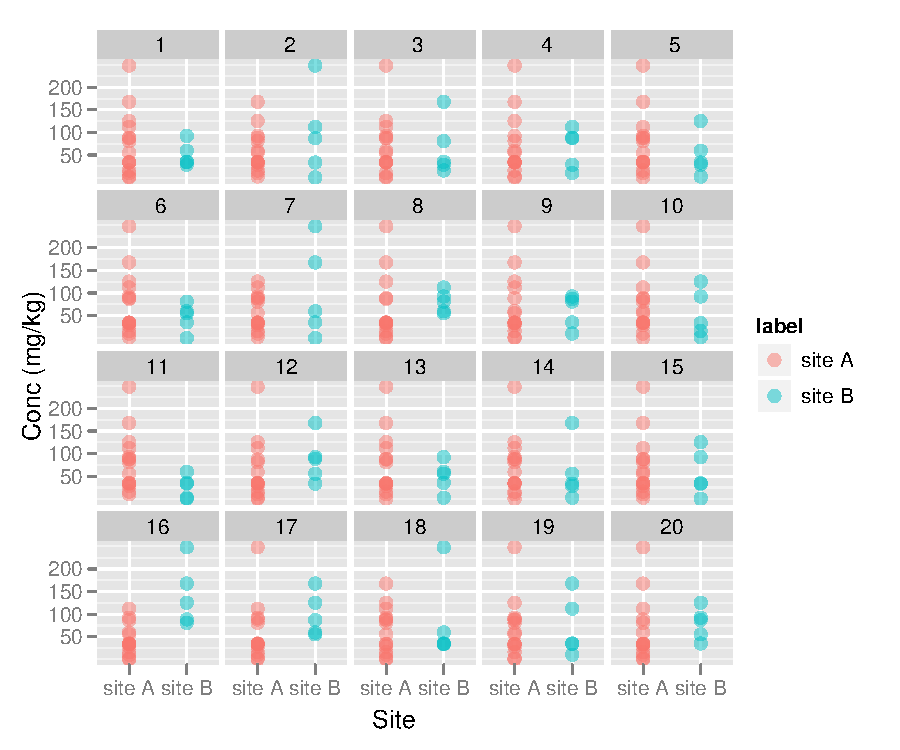
\includegraphics{lineup-dot.pdf}} \end{center}
		\end{column}
		
	\end{columns} 
	
\end{frame}

\begin{frame}
\frametitle{Comparison}
\vspace{-0.25cm}
\begin{table}[hbtp]
%\caption{Comparison of visual inference with existing inference technique}
\centering 
\begin{tabular}{p{2cm}lll} 
\hline
  &  Mathematical Inference &  Visual Inference \\ %[0.5ex] % inserts table %heading 
\hline
Hypothesis &  $H_0: \mu_1= \mu_2$ & $H_0: \mu_1 = \mu_2$\\
 & vs $H_a: \mu_1 \ne \mu_2$ & vs $H_a: \mu_1 \ne \mu_2$\\
%  \vspace{0.5cm}	
 & \begin{minipage}[h]{1cm} \begin{center} \scalebox{0.25}{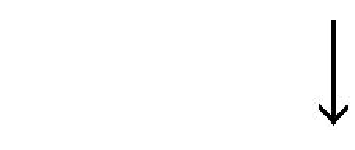
\includegraphics{down_arrow.pdf}} \end{center} \end{minipage} & \begin{minipage}[h]{1cm} \begin{center} \scalebox{0.25}{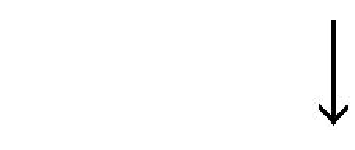
\includegraphics{down_arrow.pdf}} \end{center} \end{minipage} \\
%\vspace{0.5cm}				  
 Test Statistic & $T(y)=\frac{\bar{y}_1 - \bar{y}_2}{s\sqrt{\frac{1}{n_1} + \frac{1}{n_2}}}$ & $T(y)=$ \begin{minipage}[h]{1cm} \begin{center} \scalebox{0.2}{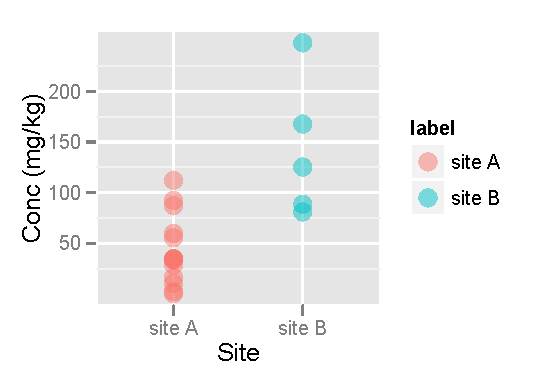
\includegraphics{data-dot.pdf}} \end{center} \end{minipage} \\
				 
 & \begin{minipage}[h]{1cm} \begin{center} \scalebox{0.25}{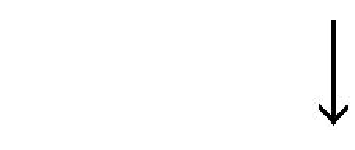
\includegraphics{down_arrow.pdf}} \end{center} \end{minipage} & \begin{minipage}[h]{1cm} \begin{center} \scalebox{0.25}{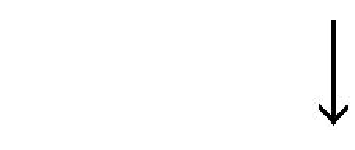
\includegraphics{down_arrow.pdf}} \end{center} \end{minipage} \\
				 
Sampling Distribution & $f_{T(y)}(t); $\begin{minipage}[h]{1cm} \begin{center} \scalebox{0.3}{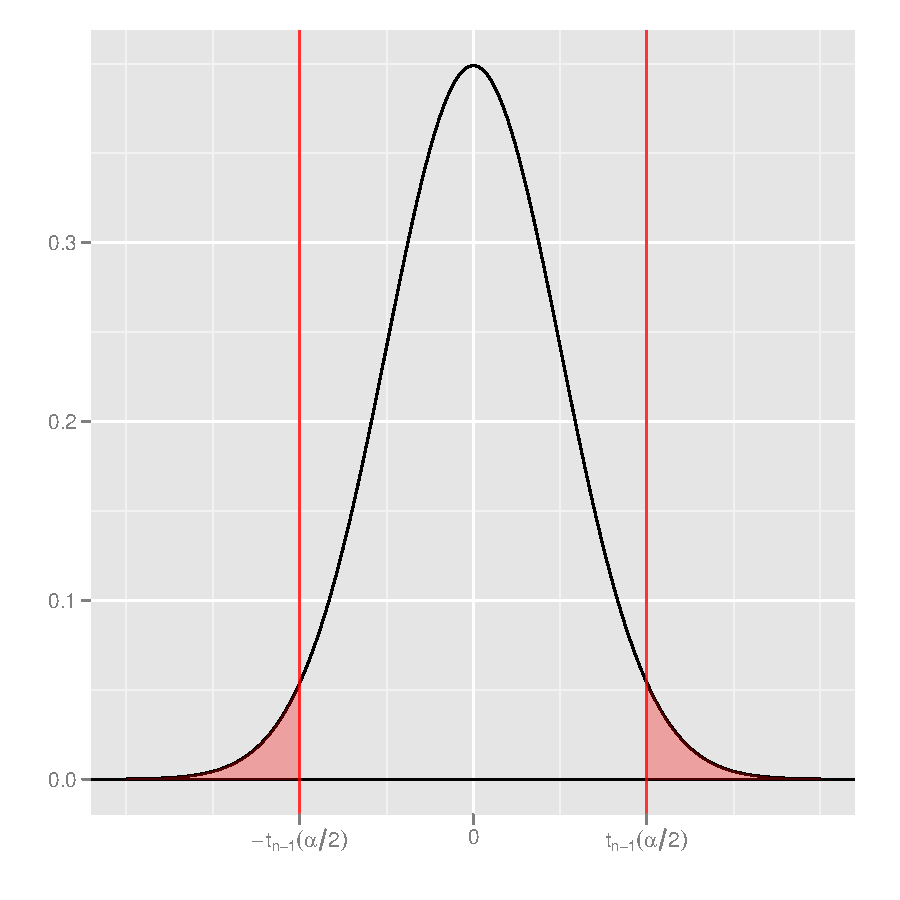
\includegraphics{two-sided-rejection.pdf}} \end{center} \end{minipage} & $f_{T(y)}(t); $ \begin{minipage}[h]{1cm} \begin{center} \scalebox{0.2}{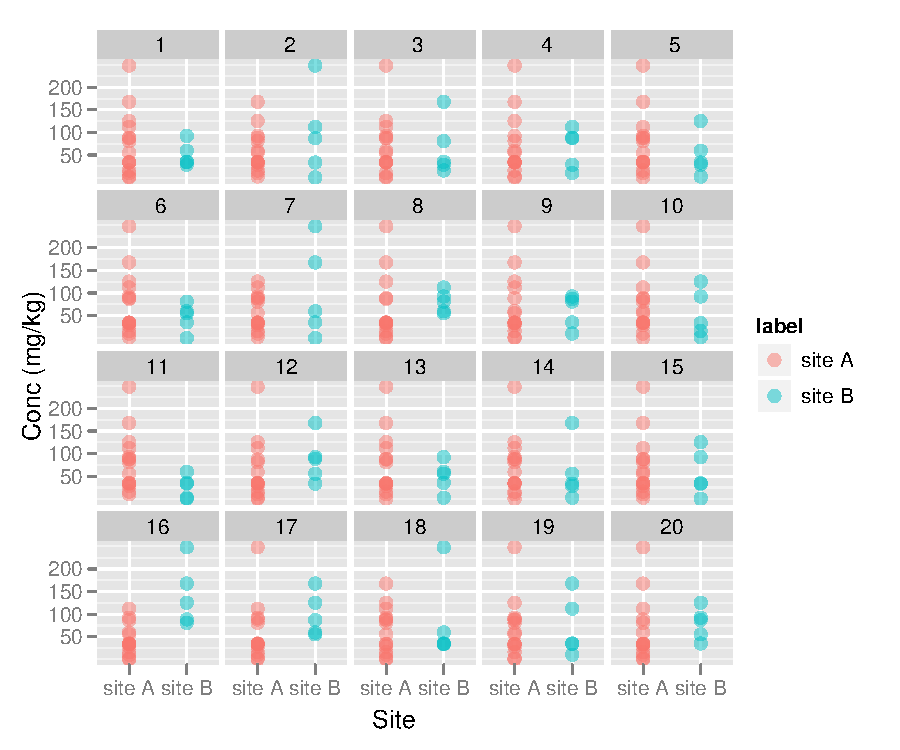
\includegraphics{lineup-dot.pdf}} \end{center} \end{minipage} \\
 & \begin{minipage}[h]{1cm} \begin{center} \scalebox{0.22}{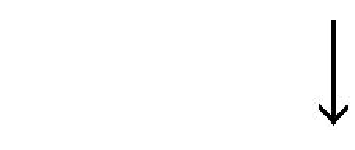
\includegraphics{down_arrow.pdf}} \end{center} \end{minipage} & \begin{minipage}[h]{1cm} \begin{center} \scalebox{0.22}{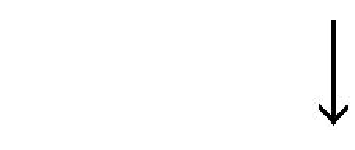
\includegraphics{down_arrow.pdf}} \end{center} \end{minipage} \\
Reject $H_0$ if & observed $T$ is extreme & observed plot is identifiable \\
\hline 
\end{tabular}
\label{tbl:compare}
\end{table}	
\end{frame}

\begin{frame}
\frametitle{Overview of the thesis}
  \begin{itemize}
    \item Visual Inference for Large $p$ Small $n$ Data.
		  \begin{itemize}
%			  \item Application of lineup protocol.
			  \item Examine the reliability of PP methods.
			  \item Check whether the separation seen in clusters are `real' or `fake'.
%			  \item power of the visual test
		  \end{itemize}
    \item Where's Waldo: Looking Closely at a Lineup.
		  \begin{itemize}
			  \item Take a closer look at the null plots in a lineup.
			  \item Develop techniques to measure the quality of a lineup.
%			  \item demonstration of the web site
		  \end{itemize}	  	  		
    \item Teaching Materials to improve Statistical Thinking.
		  \begin{itemize}
			  \item Development of teaching materials for undergraduate courses. 
			  \item Development of materials for testing the student's understanding.
%			  \item influence of demographic factors
		  \end{itemize}	  
    \item Application to Data Study.
		  \begin{itemize}
			  \item Application of lineup protocols on a large $n$ dataset.
%			  \item intend to apply the proposed methods and compare the results
		  \end{itemize}	    		  		  
  \end{itemize}		  
\end{frame}


\begin{frame}
\begin{block}{}
\begin{center} \Large{Chapter 2 --- Visual Statistical Inference for Large $p$, Small $n$ Data} \end{center}
\end{block}
\end{frame}

\begin{frame}
     \frametitle{Motivation 1 }
\begin{itemize}
\item The optimization procedure in the  \texttt{tourr} package is new, different from the algorithms that have existed before in GGobi %\cite{STLBC03} 
and XGobi. %\cite{SCB91}. 
\item  PP with the PDA index, on a large $p$, small $n$ data set from a microarray study.
\item Comparison have been looking at pure noise data. 
\item Strangely could often pick the projection of the  ``actual" data from a lineup of projections of permuted class data. 

\end{itemize}	
\end{frame}


\begin{frame}
     \frametitle{Motivation 2 }
	\begin{columns}
		\begin{column}{0.4\textwidth}
		  \begin{itemize}
		   \item $n=50$ wasps, 3 groups each having 12 wasps and the other has 14 wasp.

			  \item A subset of $p=40$ significantly different oligonucleotides from a total of 447.
			                                       \item Plot LD1 versus LD2. (Low-$d$ projection showing best separation between classes.)
			 \item F: foundress, G: gyne, Q: queen and W: worker.
			% \item Can you identify the plot of the "true" data?
		  \end{itemize}		
			
		\end{column}
		
		\begin{column}{0.6\textwidth}
			\begin{center} \scalebox{0.4}{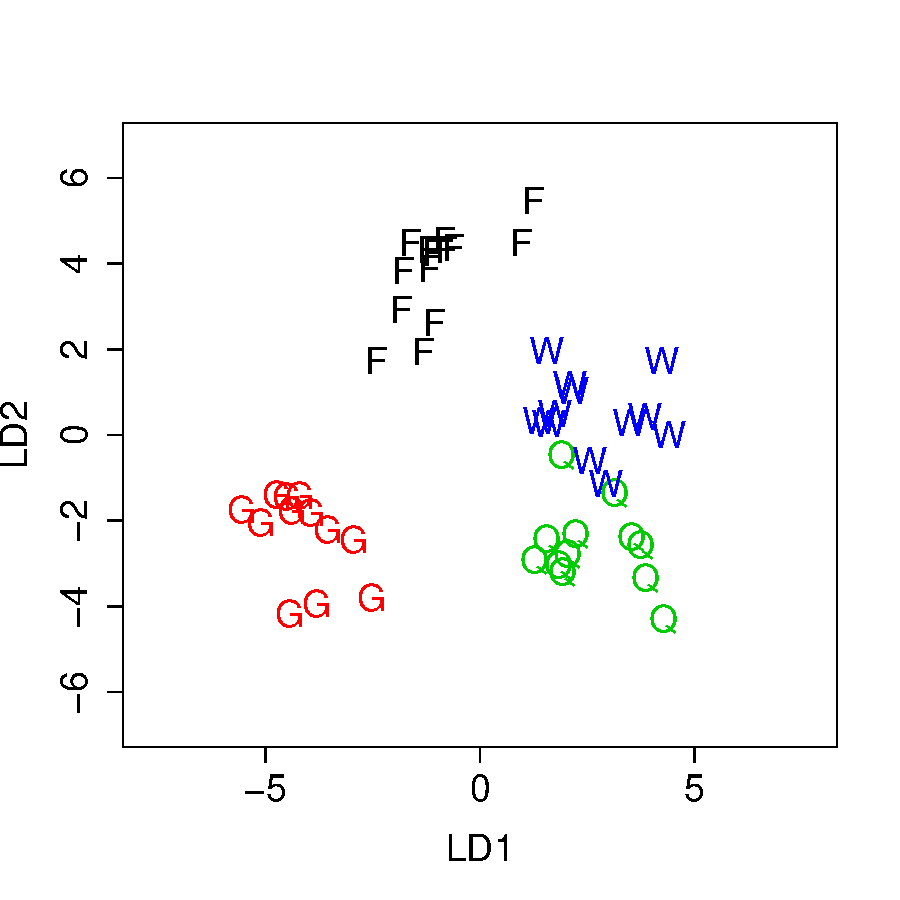
\includegraphics{toth_lda.pdf}} \end{center}
		\end{column}
	\end{columns} 
\vspace{0.05cm}

	\tiny{ Reference: ``Brain transcriptomic analysis in paper wasps identifies genes associated with behaviour across social insect lineages" by Toth {\em et. al} (Feb, 2010)}
	
\end{frame}



\begin{frame}
\frametitle{Introduction}
\begin{itemize}
\item Projection Pursuit 
			\begin{itemize}
			\item Algorithm to find the most interesting low-$d$ projections of $p$-dimensional data,  where $d \le p$.
			\item Reveals the important details about the structure of multivariate data.
			\item In this paper we used PDA index (for Large $p$, small $n$) (Lee {\em et. al} (2009) ).
			\end{itemize}		
\item \texttt{tourr} package (Wickham \& Cook (2010)) 
			\begin{itemize}
			\item Tours of multivariate data, show all low-$d$ projections of high-$p$ data.  
			\item Includes functions for creating different types of tours like grand, guided and little.
			\item Here we used the guided tour function, using the PDA index to find projections where classes are best separated.
			\end{itemize}
\end{itemize}
\end{frame}


\begin{frame}
\frametitle{Definition}
\begin{itemize}
\item Let $X_{ij}$ be the $p$-dimensional vector of the $j$-th observation in the $i$-th class, $i = 1, \dots, g$, $j = 1, \dots, n_i$.
\item $g$ is the number of classes, $n_i$ is the number of observations in class $i$ and $n = \sum_{i=1}^g n_i$.
\item $B = \sum_{i=1}^g n_i (\bar{X}_{i.} - \bar{X}_{..})(\bar{X}_{i.} - \bar{X}_{..})^T$ : between-class SS.
\item $W = \sum_{i=1}^g \sum_{j=1}^{n_i} (X_{ij} - \bar{X}_{i.})(X_{ij} - \bar{X}_{i.})^T$: within-class SS.
\item Then the LDA PP index is 
$$I_{LDA}(A) = 1 - \frac{|A^TWA|}{|A^T(W + B)A|}$$
\item $A$ is an orthogonal projection onto a $k$-dimensional space.
\end{itemize}
\end{frame}

\begin{frame}
\begin{itemize}
\item The LDA index finds a projection $a$ by maximizing $a^T\sum_Ba/a^T\sum_Wa$.
\item $\sum_B$ is the between-class covariance matrix and $\sum_W$ is the within-class covariance matrix.
\item For small $n$ and large $p$, for some $a$, $a^T\sum_Wa$ tends to be very small.
\item PDA index is an improvement over LDA index.
\item The PDA index is
$$I_{PDA}(A, \lambda) = 1 - \frac{|A^T\{(1 - \lambda)W^s + n\lambda I_p\}A|}{|A^T\{(1 - \lambda)(B^s + W^s) + n\lambda I_p\}A|}$$
\item $W^s$ and $B^s$ is the within-class and between-class sum of squares of the standardized data respectively.
\end{itemize}
\end{frame}

%\begin{frame}
%  \frametitle{Checking PP optimization}
%	\begin{columns}
%		\begin{column}{0.4\textwidth}{1D projections}
%		  \begin{itemize}
%			  \item Data simulated from a standard normal with $n=30, p=100$.
%			  \item The first 15 observations labelled class 1, last 15 labelled class 2
%			 -- {\bf No true class}, data is pure noise.
%%			\item Can you identify the plot of the ``true" data?
%		  \end{itemize}		
%			
%		\end{column}
%		
%		\begin{column}{0.6\textwidth}
%			 \begin{center} \scalebox{0.5}{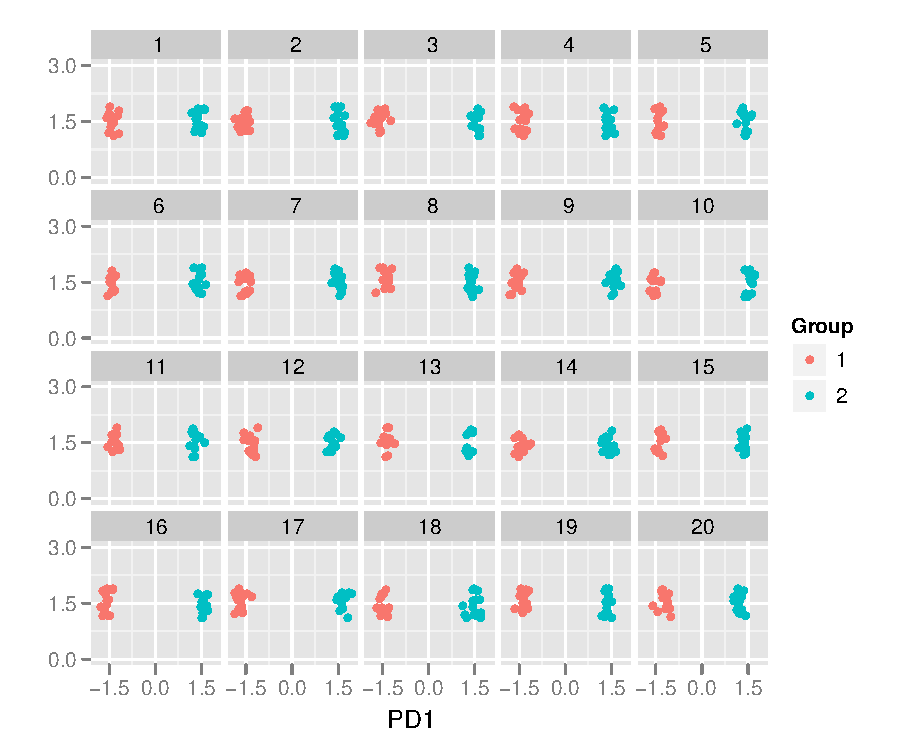
\includegraphics{plot_1d_100_4.pdf}} \end{center}
%		\end{column}
%	\end{columns}  
%\end{frame} 
%
%
%\begin{frame}
%  \frametitle{ 1D projections}
%	\begin{columns}
%		\begin{column}{0.4\textwidth}
%		  \begin{itemize}
%			  \item Data simulated from a standard normal with $n=30, p=100$.
%			  \item 99 dimensions of pure noise and 1 dimension means of class 1, 2 are different -- {\bf there is a ``true" class}.
%%			\item Can you identify the plot of the ``true" data?
%		  \end{itemize}		
%			
%		\end{column}
%		
%		\begin{column}{0.6\textwidth}
%			 \begin{center} \scalebox{0.5}{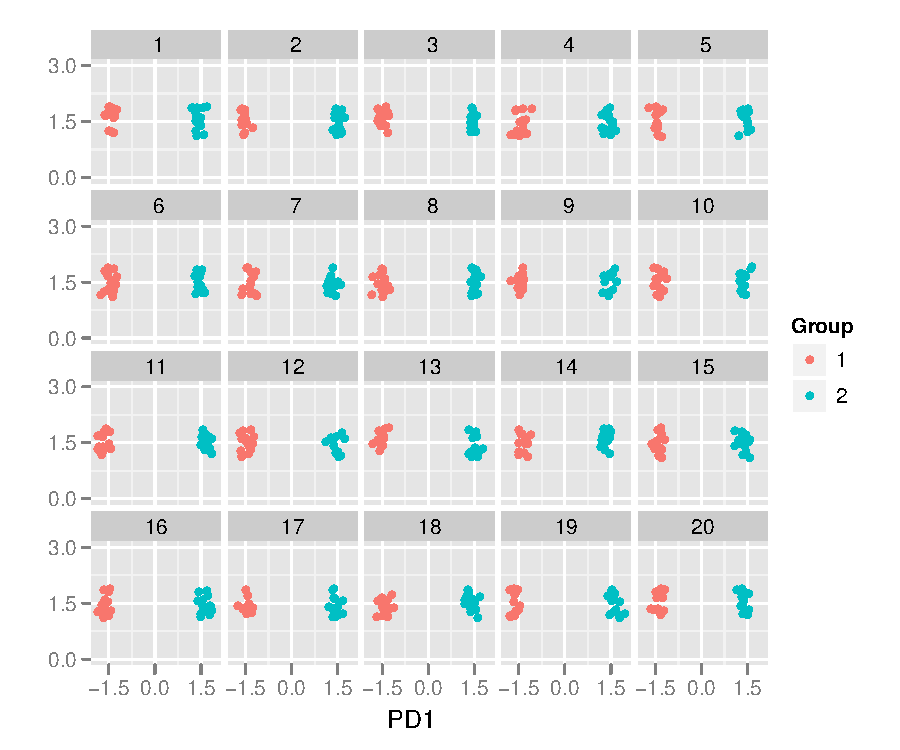
\includegraphics{plot_1d_99_19.pdf}} \end{center}
%		\end{column}
%	\end{columns}  
%\end{frame} 
%

\begin{frame}
  \frametitle{ 2D projections}
	\begin{columns}
		\begin{column}{0.4\textwidth}
		  \begin{itemize}
			  \item Data simulated from a standard normal with $n=30, p=100$.
			  \item The first 10 observations labelled class 1, the second 10 class 2 and the last 10 class 3. 
			 -- {\bf No true class}, data is pure noise.
			\item 19 null plots of 30 generated with the smallest Wilks' $\lambda$ value was used. 
			\item Also did for 1D projections.
%			\item Can you identify the plot of the "true" data?
		  \end{itemize}		
			
		\end{column}
		
		\begin{column}{0.6\textwidth}
			 \begin{center} \scalebox{0.5}{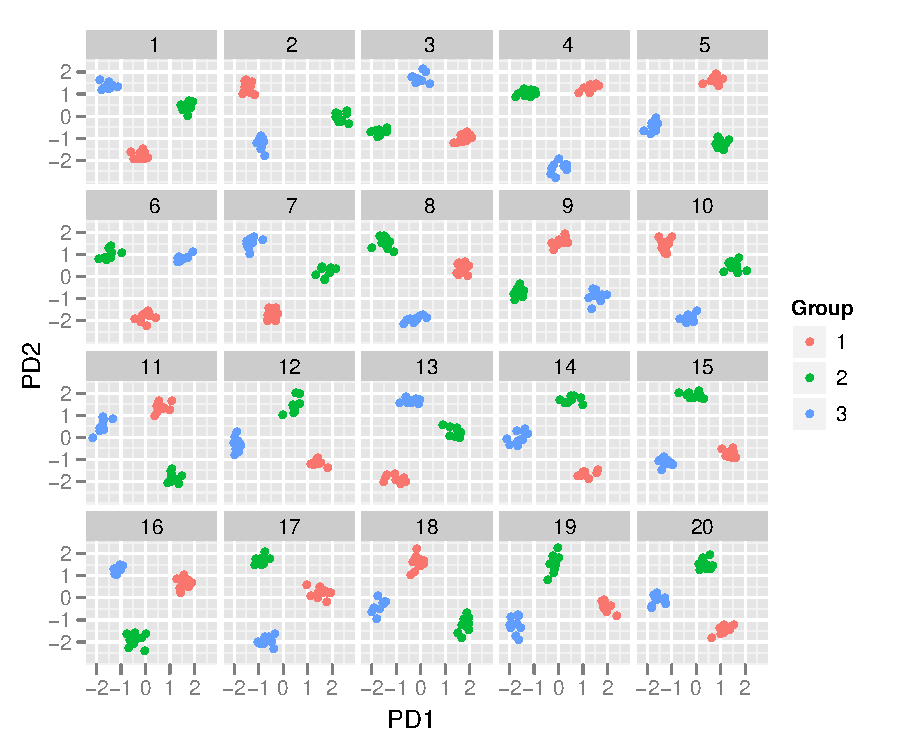
\includegraphics{plot_2d_100_15.pdf}} \end{center}
		\end{column}
	\end{columns}  
\end{frame} 


\begin{frame}
  \frametitle{ 2D projections}
	\begin{columns}
		\begin{column}{0.4\textwidth}
		  \begin{itemize}
			  \item Data simulated from a standard normal with $n=30, p=100$ but 98 dimensions of pure noise and 2 dimensions of real separation -- there is  {\bf true class} separation.
			\item 19 null plots of 30 generated with the smallest Wilks' $\lambda$ value was used. 
			\item Also did for 1D projections.
%			\item Can you identify the plot of the ``true" data?
		  \end{itemize}		
			
		\end{column}
		
		\begin{column}{0.6\textwidth}
			 \begin{center} \scalebox{0.5}{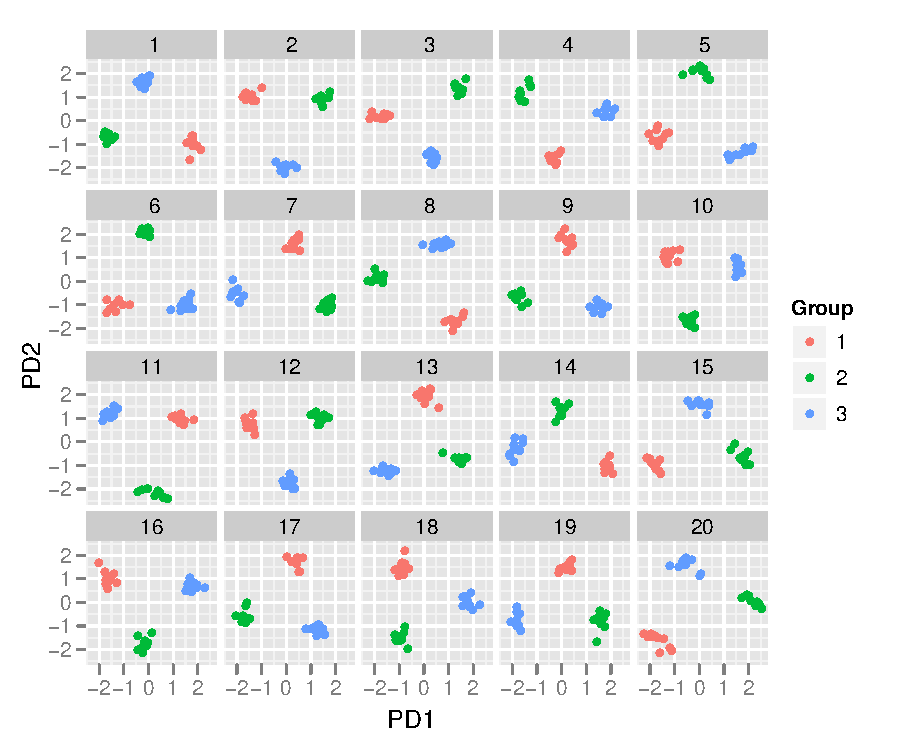
\includegraphics{plot_2d_98_5.pdf}} \end{center}
		\end{column}
	\end{columns}  
\end{frame} 

\begin{frame}
  \frametitle{Results}
	\begin{columns}
		\begin{column}{0.45\textwidth}
		  \begin{itemize}
			  \item 5 lineups of each scenario were made and showed to each of the authors, who did not know which scenario was used.
		\item Proportion ``true'' data is selected.
		\begin{table}[ht]
		\begin{center}
		\begin{tabular}{c|cc}
  		\hline
 		& noise & not noise\\
 	 	\hline
		1D &  20\% & 90\% \\ 
		2D &  30\% & 60\% \\
   		\hline
		\end{tabular}
		\end{center}
		\end{table}
	
	%	\begin{itemize}	  
			 \item People are more often correct in selecting the true plot when there is some real separation.
		  \end{itemize}		
			
		\end{column}
		
		\begin{column}{0.55\textwidth}
			 \begin{center} 
			\scalebox{0.2}{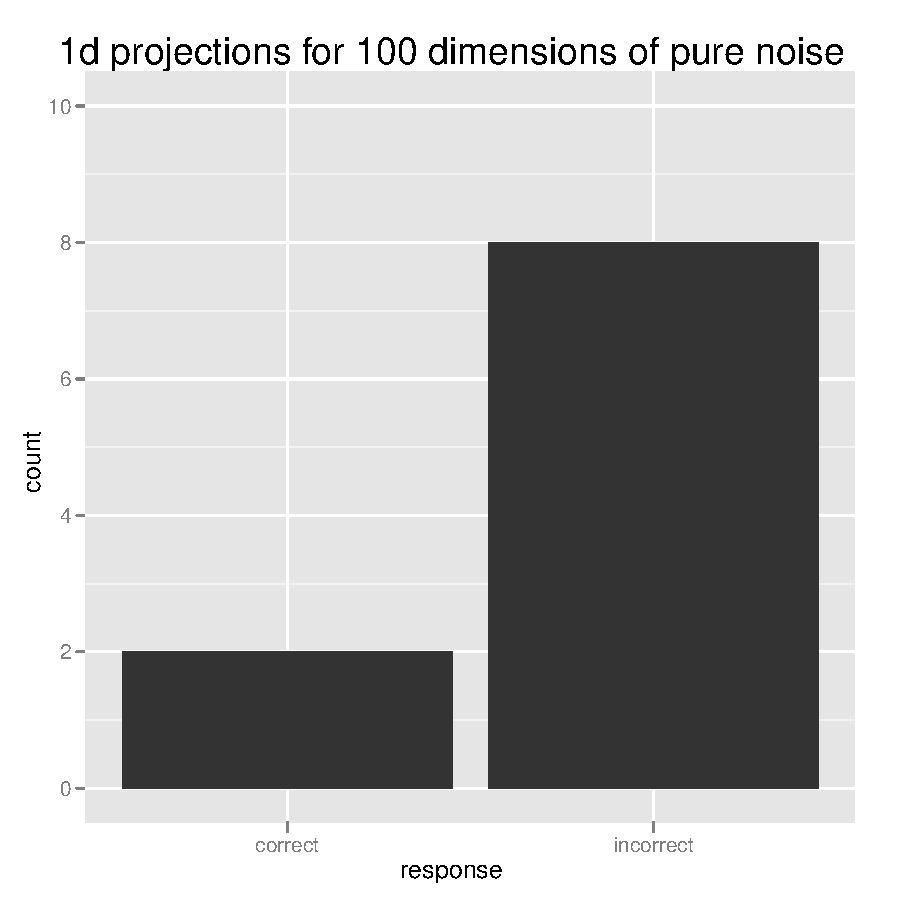
\includegraphics{result_1d_noise.pdf}} 
			\scalebox{0.2}{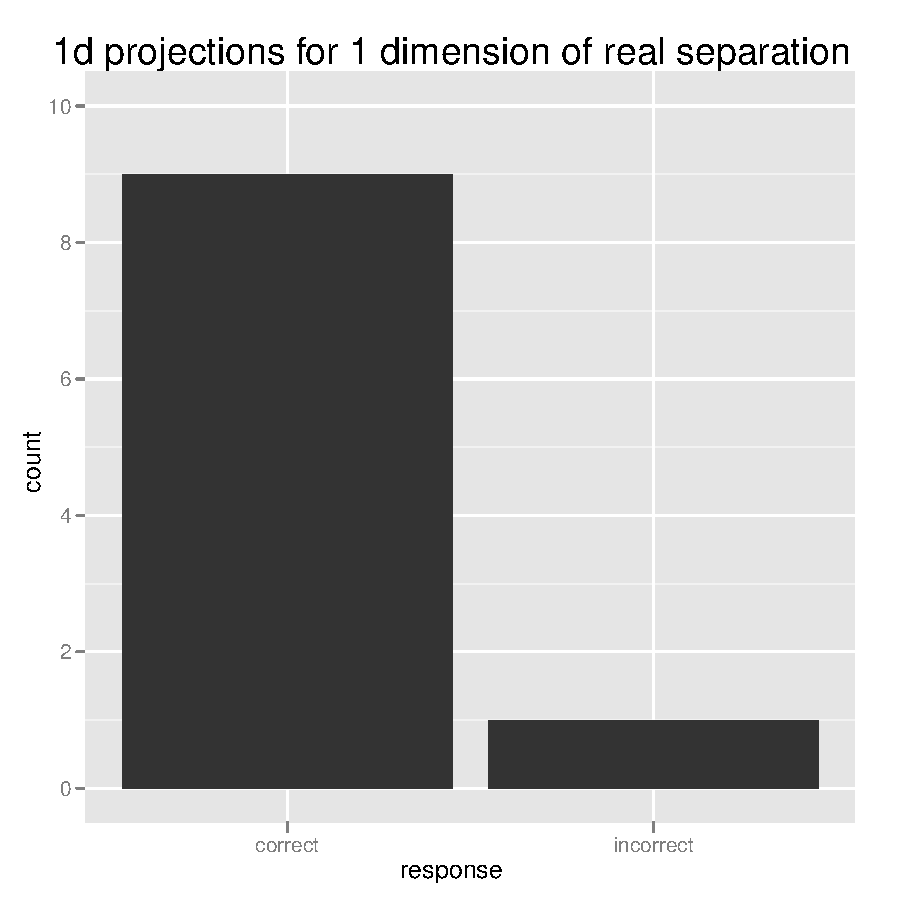
\includegraphics{result_1d_sep.pdf}}
			\scalebox{0.2}{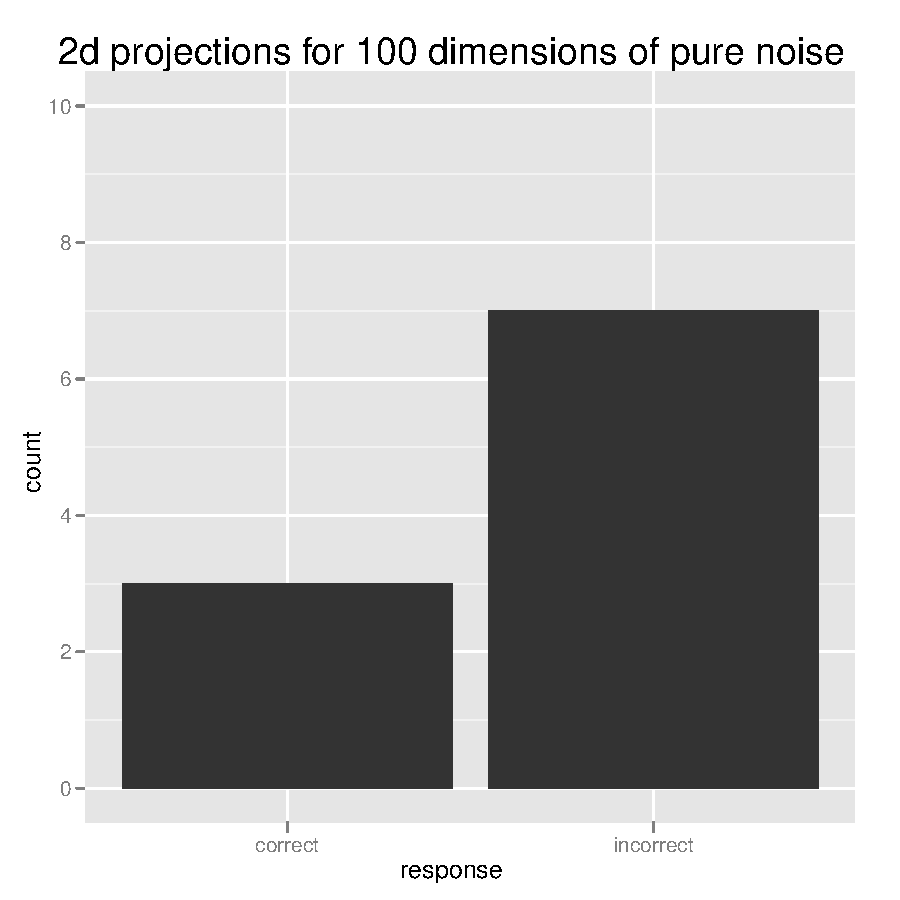
\includegraphics{result_2d_noise.pdf}}
			\scalebox{0.2}{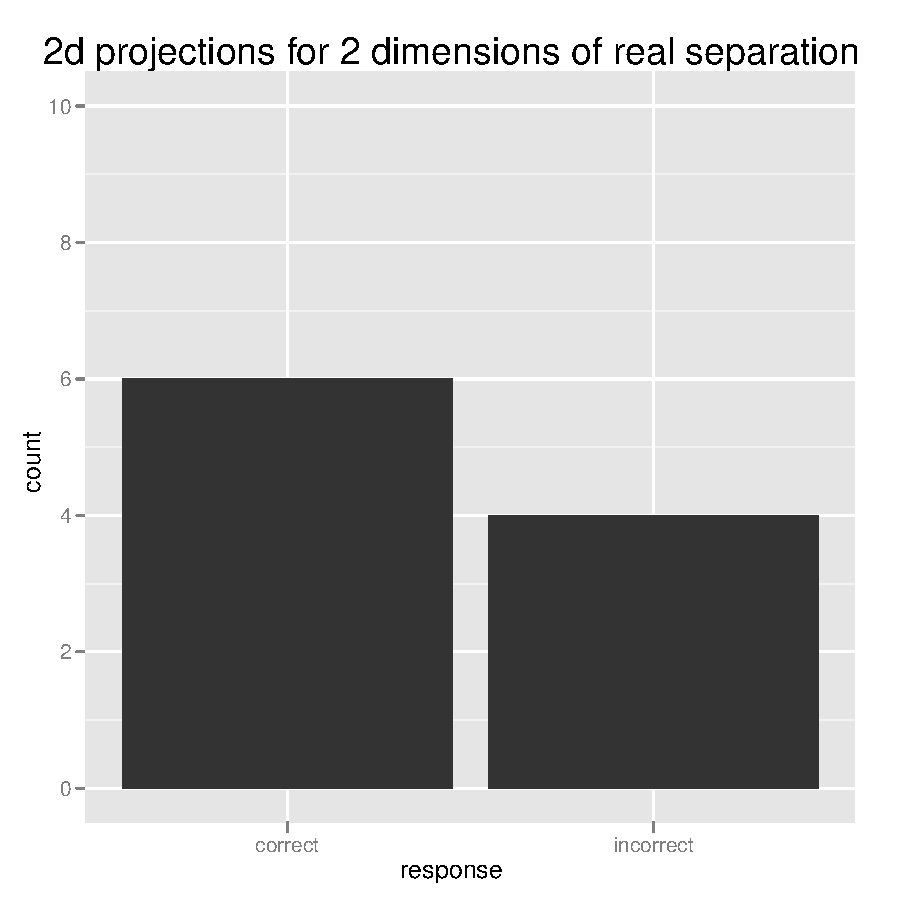
\includegraphics{result_2d_sep.pdf}}
			\end{center}
		\end{column}
	\end{columns}  
\end{frame}

\begin{frame}
\frametitle{Distance Increasing with $p$ for Fixed $n$}
\begin{itemize}
\item Data simulated from a standard normal with $n=30$. 
%\item Data divided into 2 classes, first 15 class 1, second 15 class 2.
\item Plot 1D and 2D projections showing best separation each time. 
\item We increase the number of dimensions ($p$) by 1 each time. %\item Repeat 100 times!
\end{itemize}
\begin{center}
\scalebox{0.18}{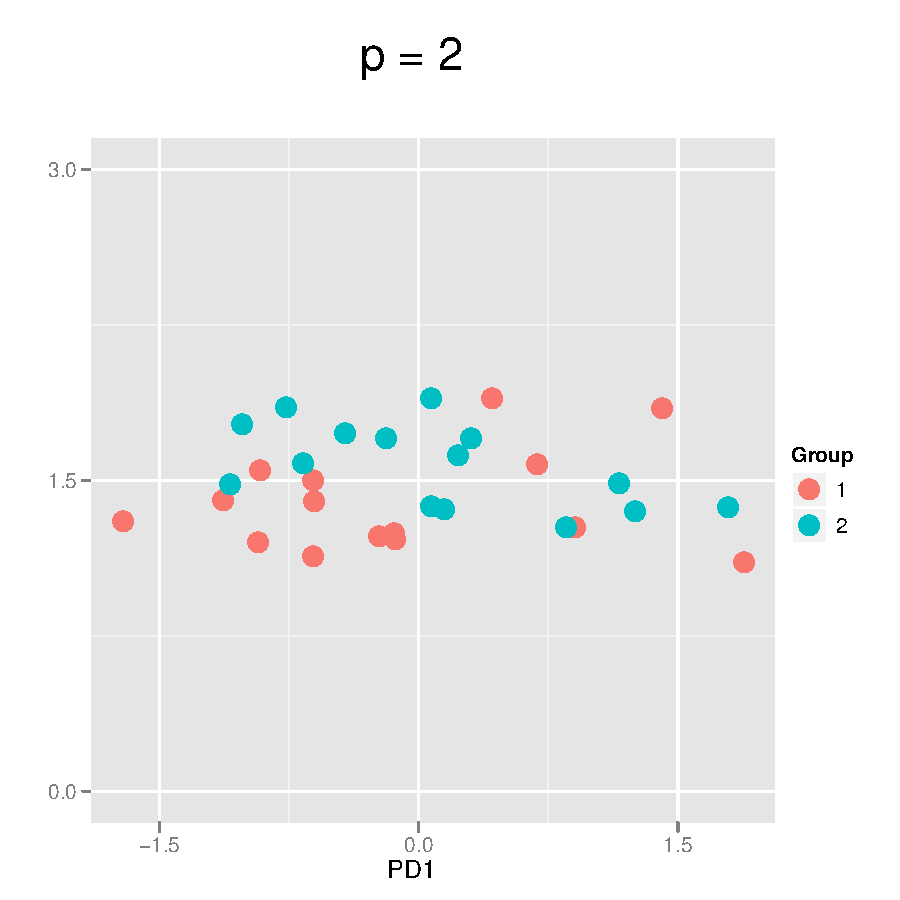
\includegraphics{plot_1d_2.pdf}}
\scalebox{0.18}{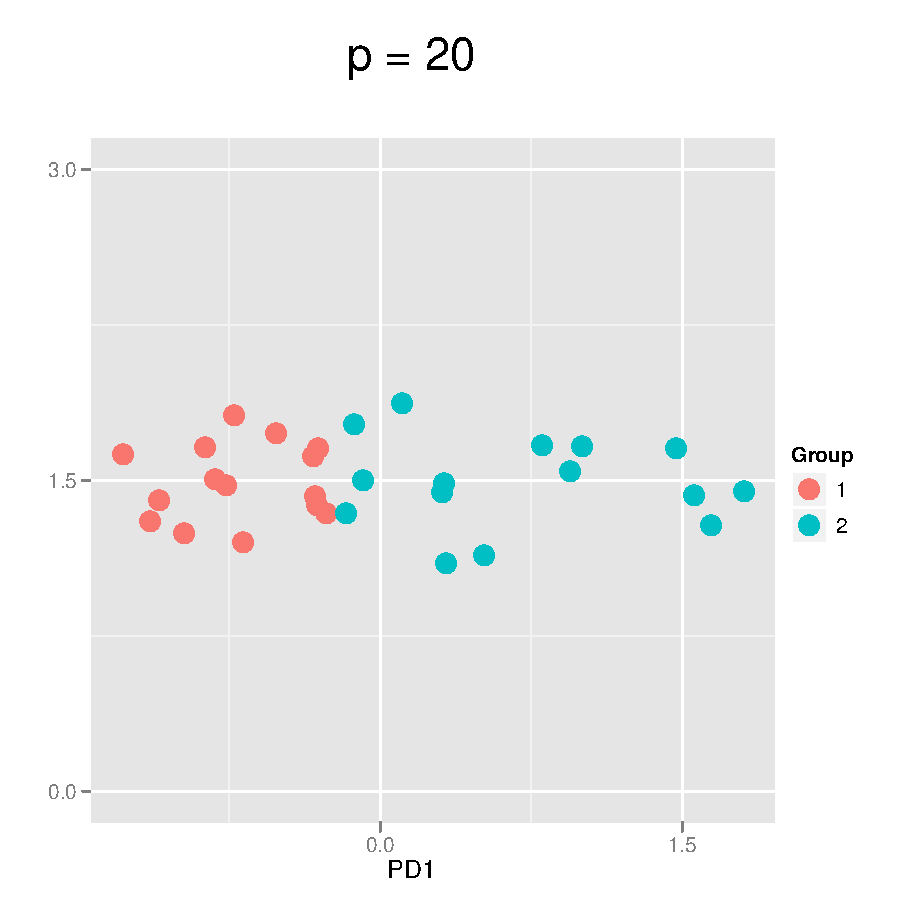
\includegraphics{plot_1d_20.pdf}}
\scalebox{0.18}{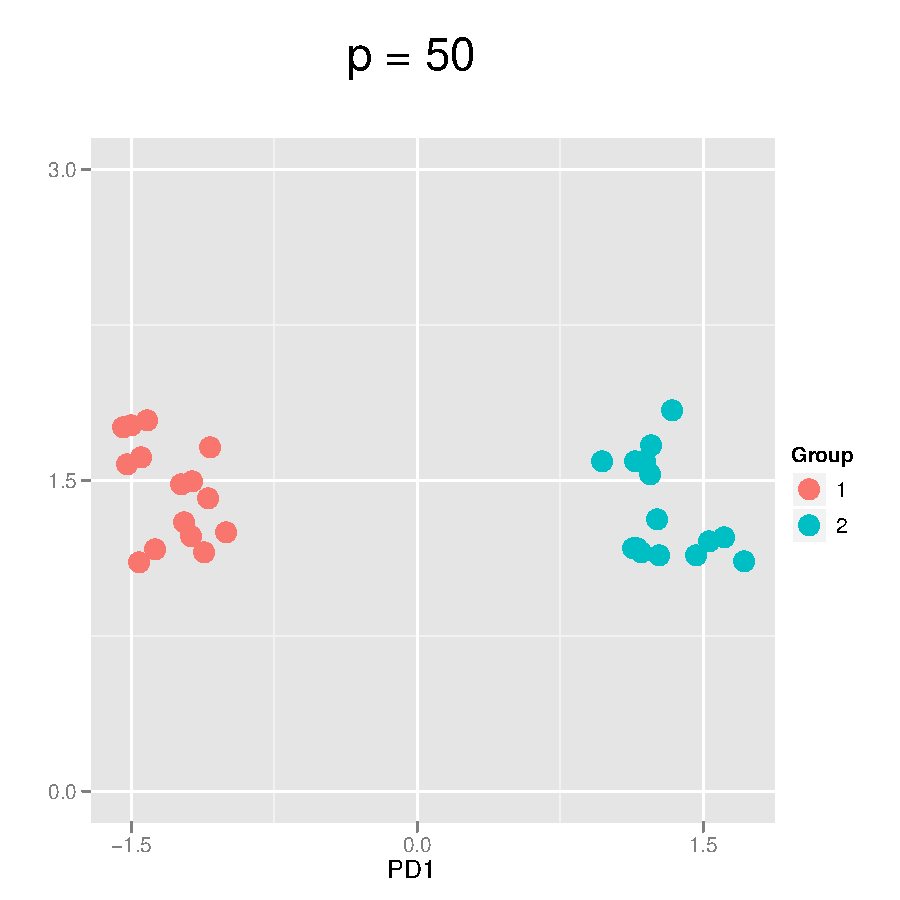
\includegraphics{plot_1d_50.pdf}}
\scalebox{0.18}{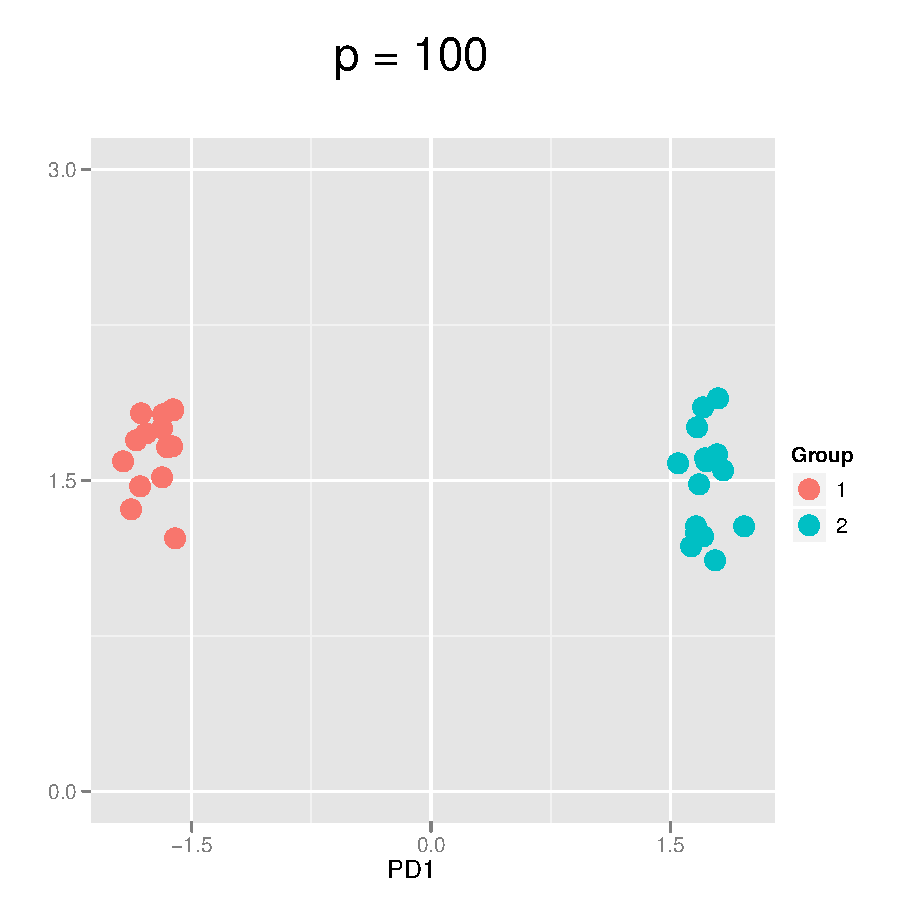
\includegraphics{plot_1d_100.pdf}}
\scalebox{0.18}{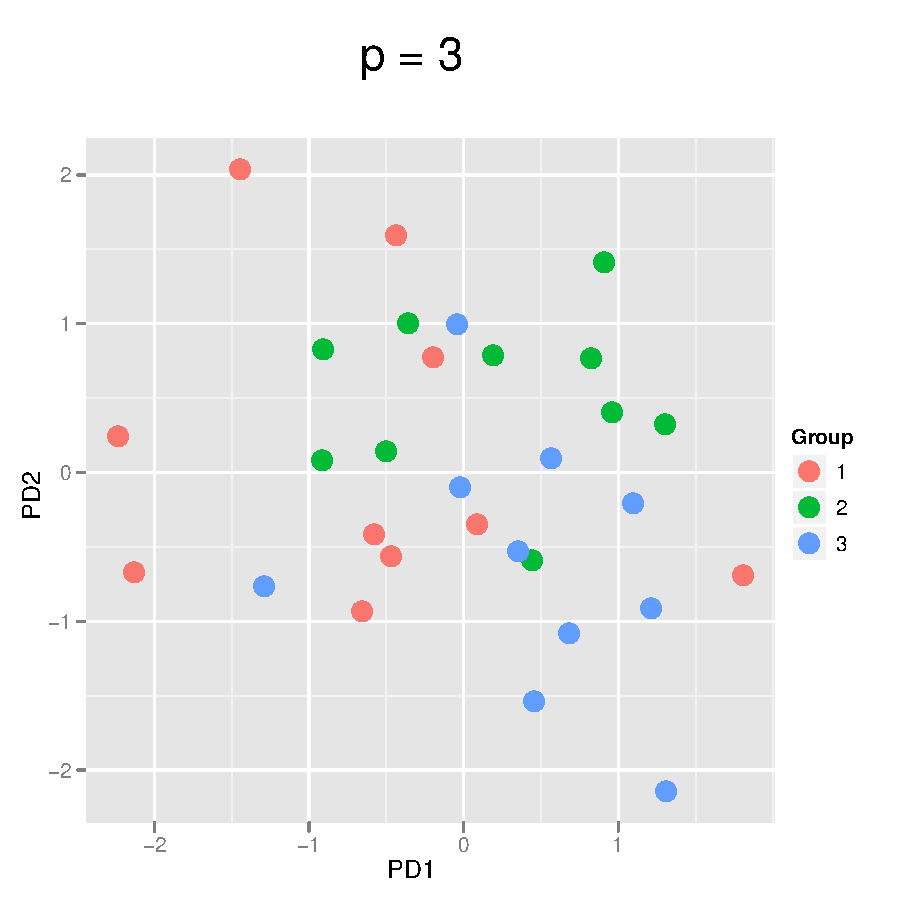
\includegraphics{plot_2d_3.pdf}}
\scalebox{0.18}{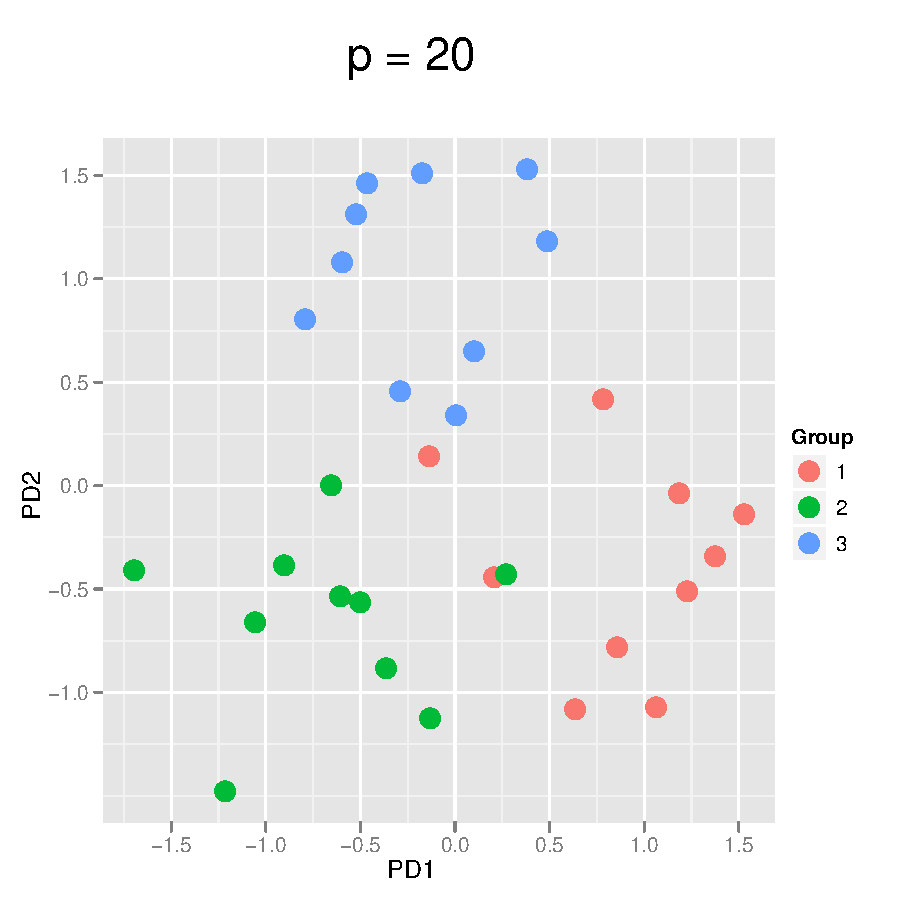
\includegraphics{plot_2d_20.pdf}}
\scalebox{0.18}{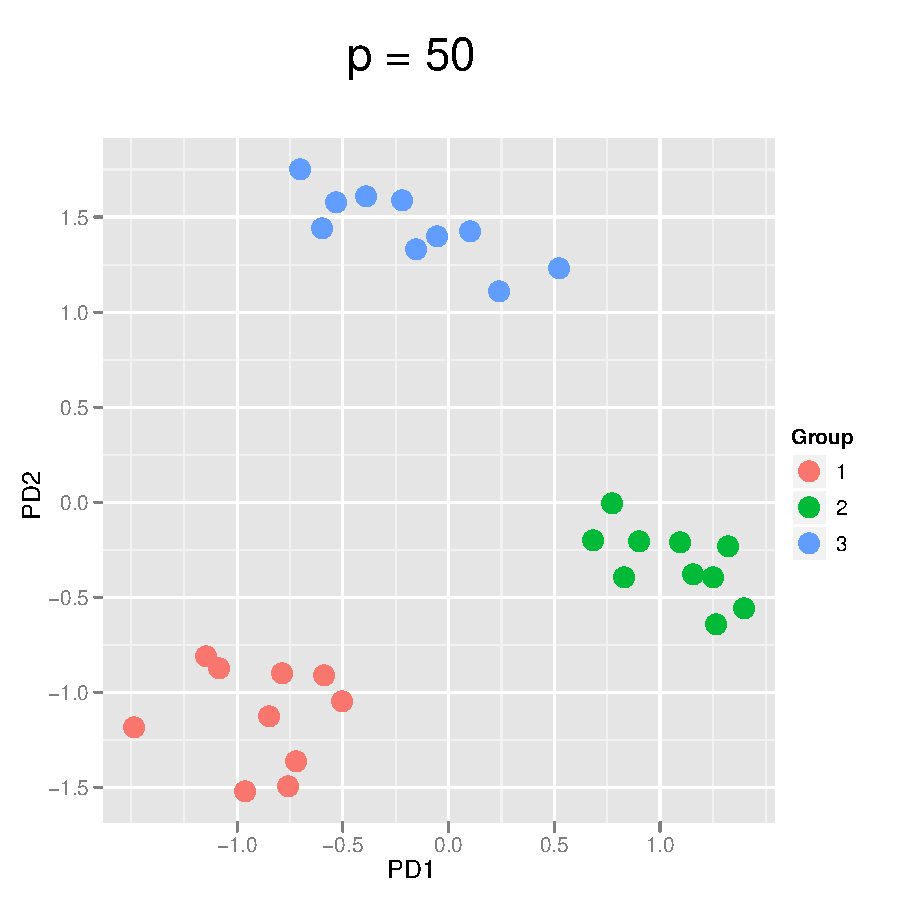
\includegraphics{plot_2d_50.pdf}}
\scalebox{0.18}{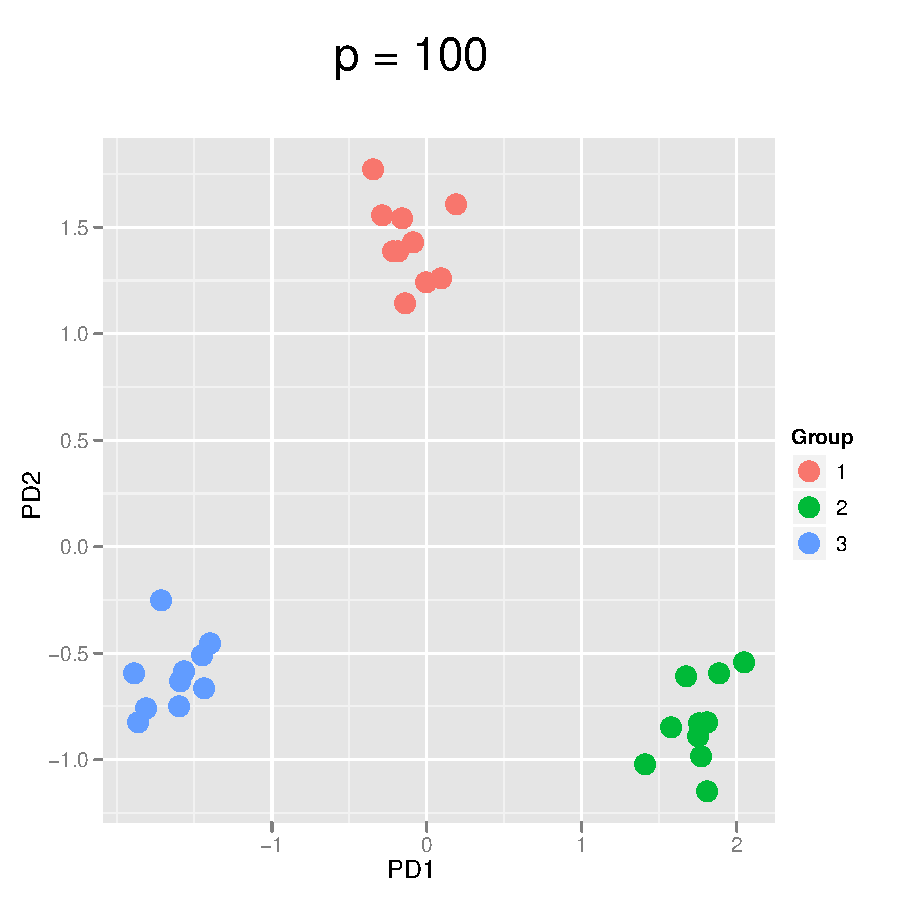
\includegraphics{plot_2d_100.pdf}}
\end{center}
\end{frame}

%\begin{frame}
%\frametitle{Distance Increasing with $p$ for Fixed $n$}
%\begin{itemize}
%\item Data simulated from a standard normal with $n=30$. 
%\item Data divided into 3 classes, randomly, 10 observations in each class.
%\item Plot two dimensional projections showing best separation each time.
%\item Starting from $p=3$ we increase the number of dimensions ($p$)  by 1 each time. %, and ask observer to say when the classes are actually separated. 
%%\item Repeat 100 times!
%\end{itemize}
%\begin{center}
%\scalebox{0.18}{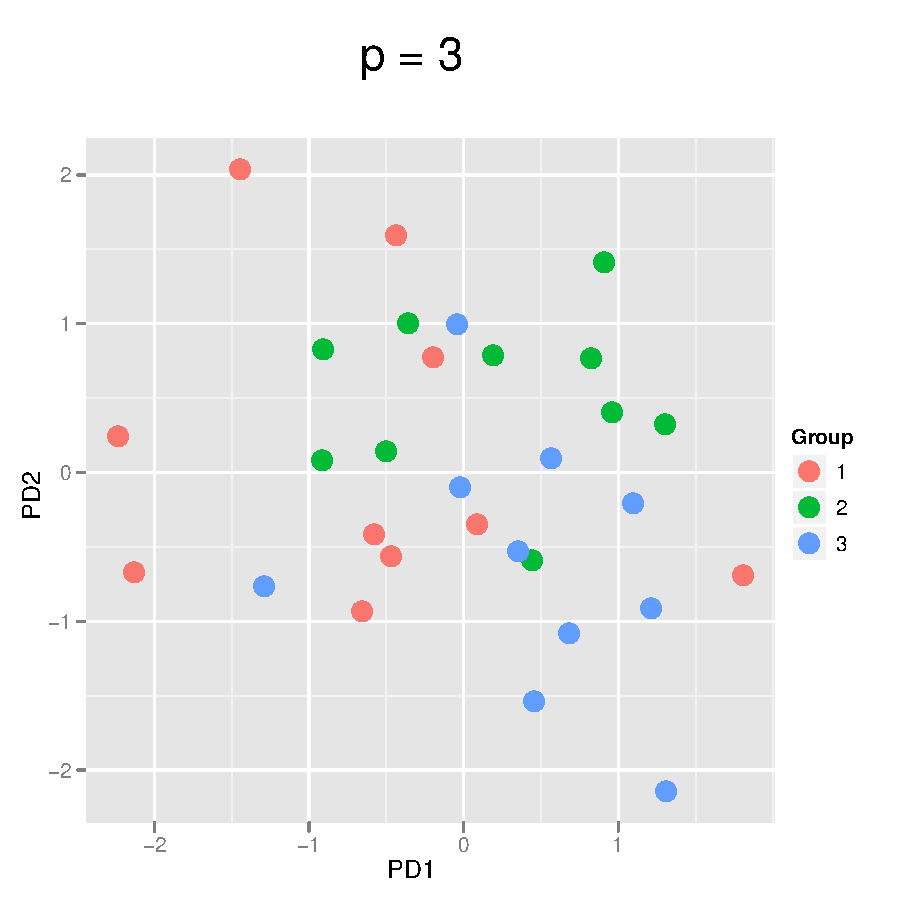
\includegraphics{plot_2d_3.pdf}}
%\scalebox{0.18}{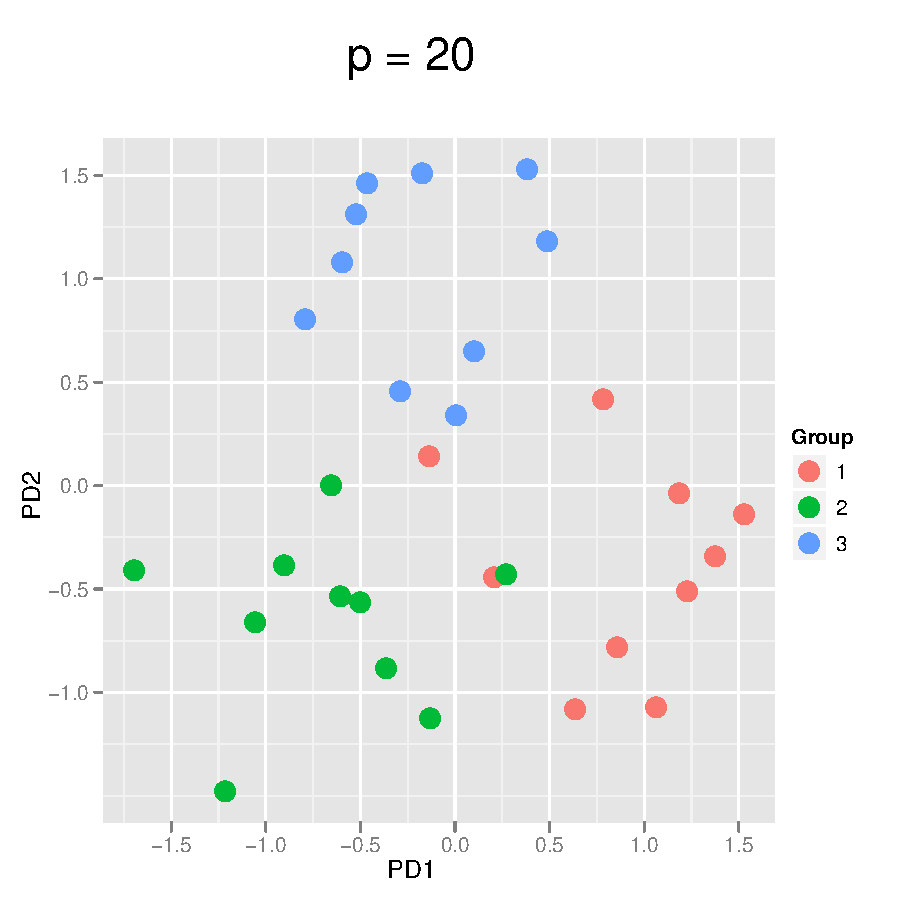
\includegraphics{plot_2d_20.pdf}}
%\scalebox{0.18}{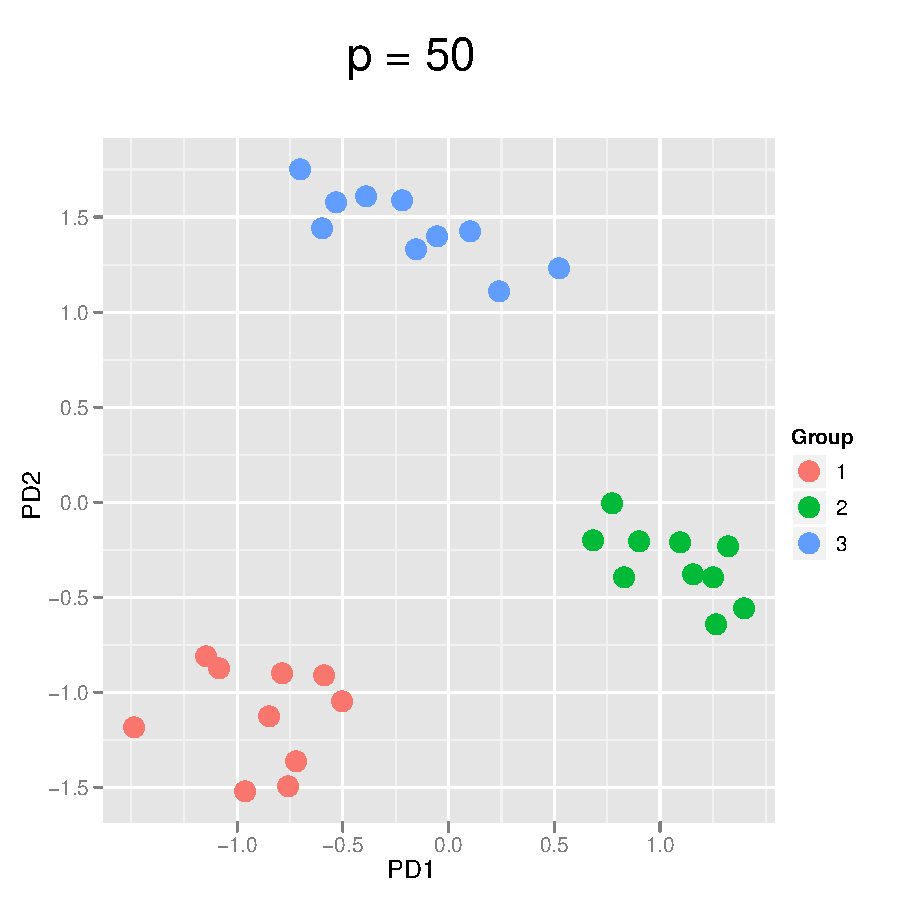
\includegraphics{plot_2d_50.pdf}}
%\scalebox{0.18}{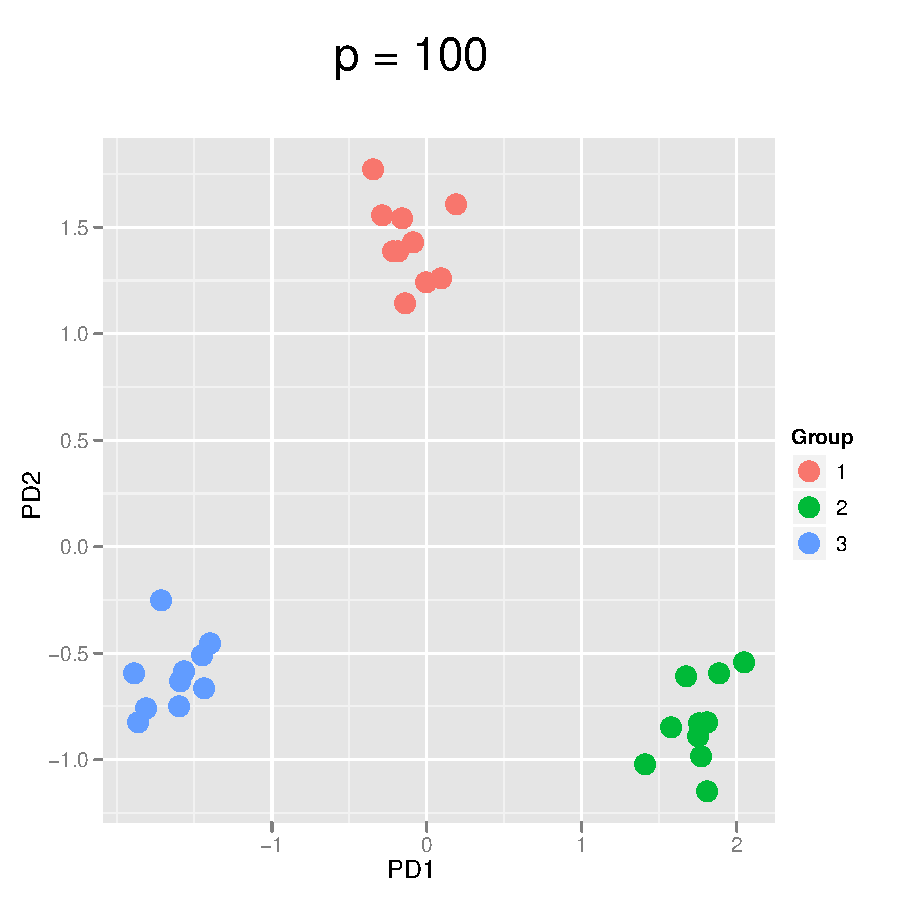
\includegraphics{plot_2d_100.pdf}}
%\end{center}
%\end{frame}

\begin{frame}
\frametitle{Observations}
\begin{itemize}
\item The distance between the clusters increases as the number of dimensions increases.
\item There is no true class -- it is pure noise data -- any separation seen between classes in the projection are purely due to the high dimensions.
%\item Motivated to calculate the 90\% confidence interval of the number of dimension at which the classes start separating out for both 1D and 2D projections.
\end{itemize}
\end{frame}


%\begin{frame}
%\frametitle{90\% Confidence Interval}
%\begin{itemize}
%\item Consider $n=30$ observations with 2 classes for 1D projections and 3 classes for 2D projections.
%\item Plot 1D projections for $p$ ranging from 2 to 62.
%\item Plot 2D projections for $p$ from 3 to 62.
%\item Repeat 100 times. 
%\end{itemize}
%\end{frame}

%\begin{frame}
%\frametitle{90\% Confidence Interval}
%	\begin{columns}
%		\begin{column}{0.5\textwidth}
%		\begin{itemize}
%		\item 1D projections. \item Fixed $n=30$. \item $5^{th}$ and $95^{th}$ percentiles give $p$ between 24 to 34.
%		\end{itemize}
%		%\begin{center} 
%		\scalebox{0.4}{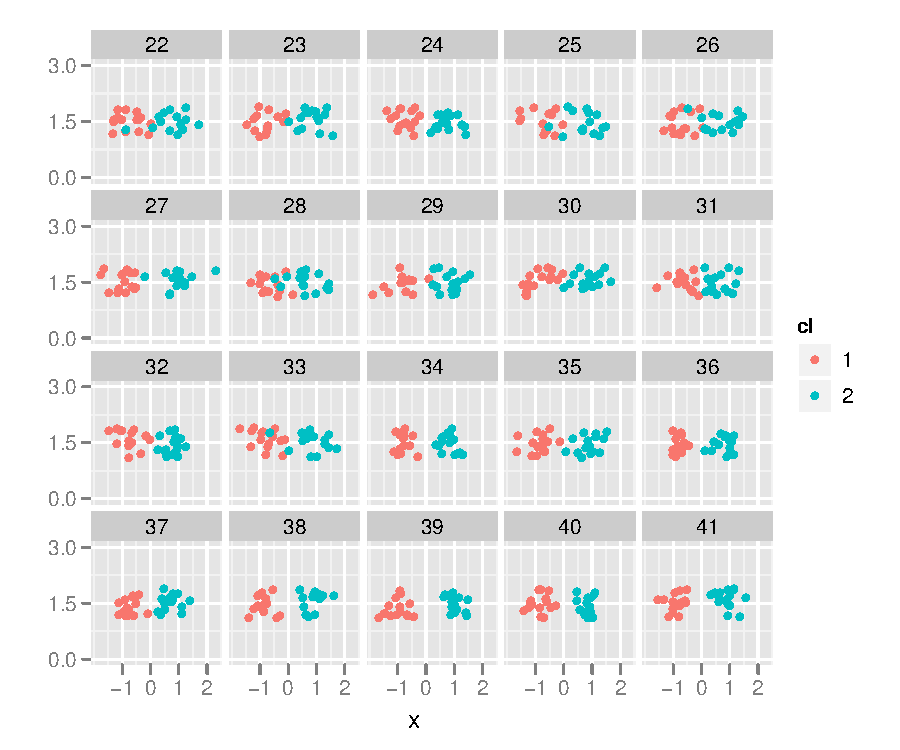
\includegraphics{npratio22_41_new.pdf}} 
%		%\end{center}	
%		\end{column}
%		
%		\begin{column}{0.5\textwidth}
%		\begin{itemize}
%		\item 2D projections. \item Fixed $n=30$. \item $5^{th}$ and $95^{th}$ percentiles give $p$ between 26 to 36.
%		\end{itemize}
%		%\begin{center} 
%		\scalebox{0.4}{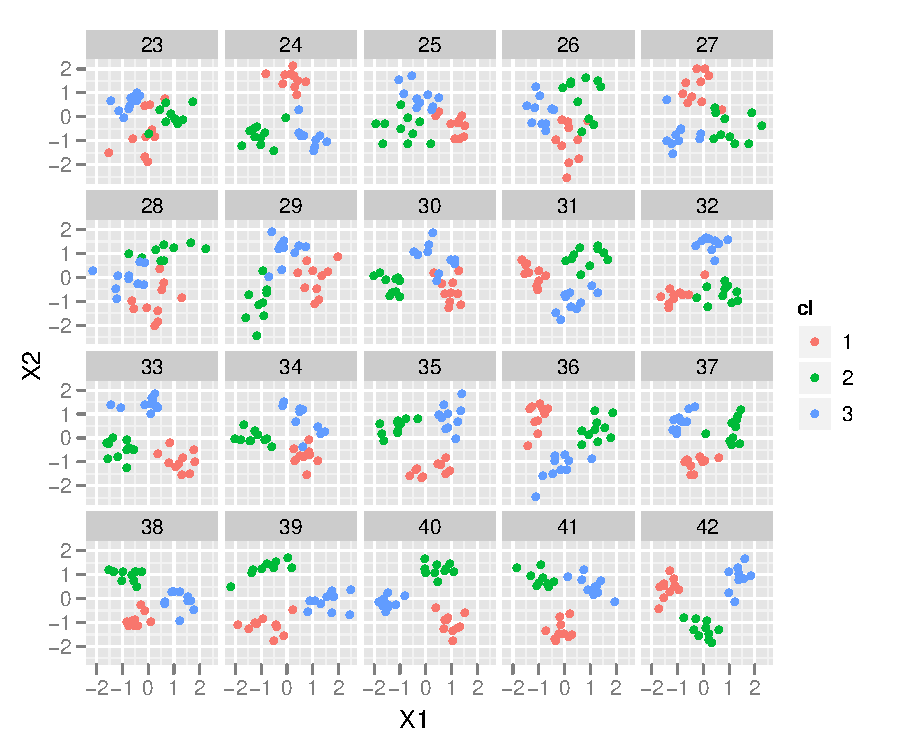
\includegraphics{npratio23_42_new.pdf}} 
%		%\end{center}
%		\end{column}
%	\end{columns}  
%\end{frame}


\begin{frame}
	\frametitle{LDA of the Paper Wasp Dataset (New Work)}
	\begin{columns}
		\begin{column}{0.4\textwidth}
		  \begin{itemize}
		  	\item Obtained the wasp data from the authors. 
			  \item Perform PP using a LDA index.
			\item Plot LD1 vs LD2 of the $p=40$ significantly different oligonucleotides from a total of 447.
			 \item Generate a lineup by permuting the group variable. 
 
%			\item Can you identify the plot of the ``true" data?
		  \end{itemize}		
			
		\end{column}
		
		\begin{column}{0.6\textwidth}
			 \begin{center} \scalebox{0.5}{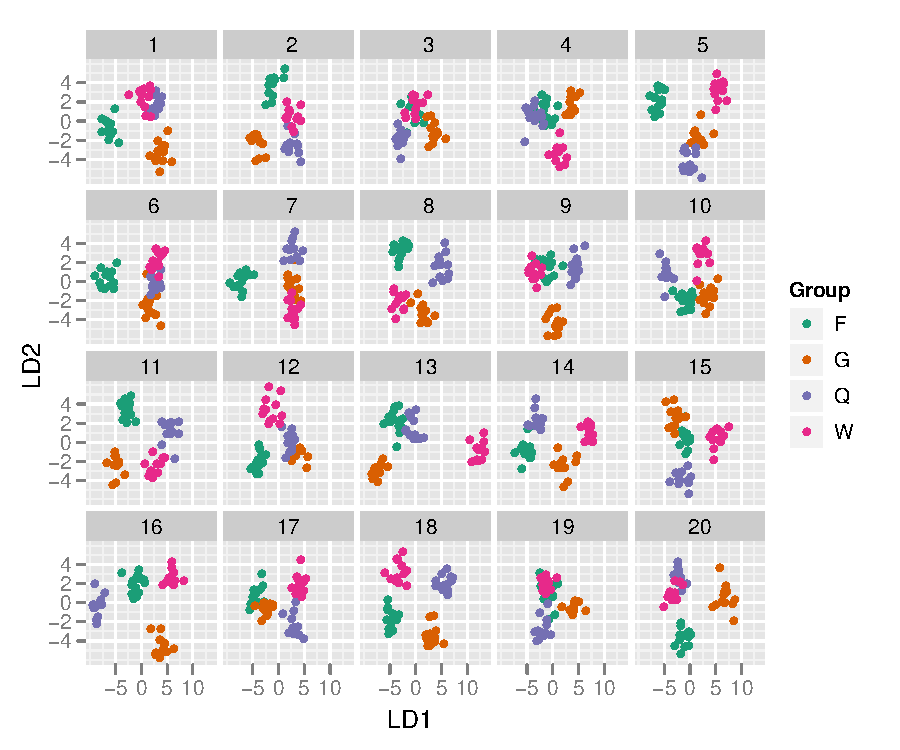
\includegraphics{toth_lineup_lda.pdf}} \end{center}
		\end{column}
	\end{columns}  

\end{frame}

\begin{frame}
	\frametitle{PDA of the Paper Wasp Dataset (New Work) }
	\begin{columns}
		\begin{column}{0.4\textwidth}
		  \begin{itemize}
%		  	\item Obtained the wasp data from the authors. 
			  \item Perform PP using a PDA index.
			\item Plot PD1 vs PD2 of the $p=40$ significantly different oligonucleotides from a total of 447.
			  \item Generate a lineup by permuting the group variable. 
%			\item Can you identify the plot of the ``true" data?
		  \end{itemize}		
			
		\end{column}
		
		\begin{column}{0.6\textwidth}
			 \begin{center} \scalebox{0.5}{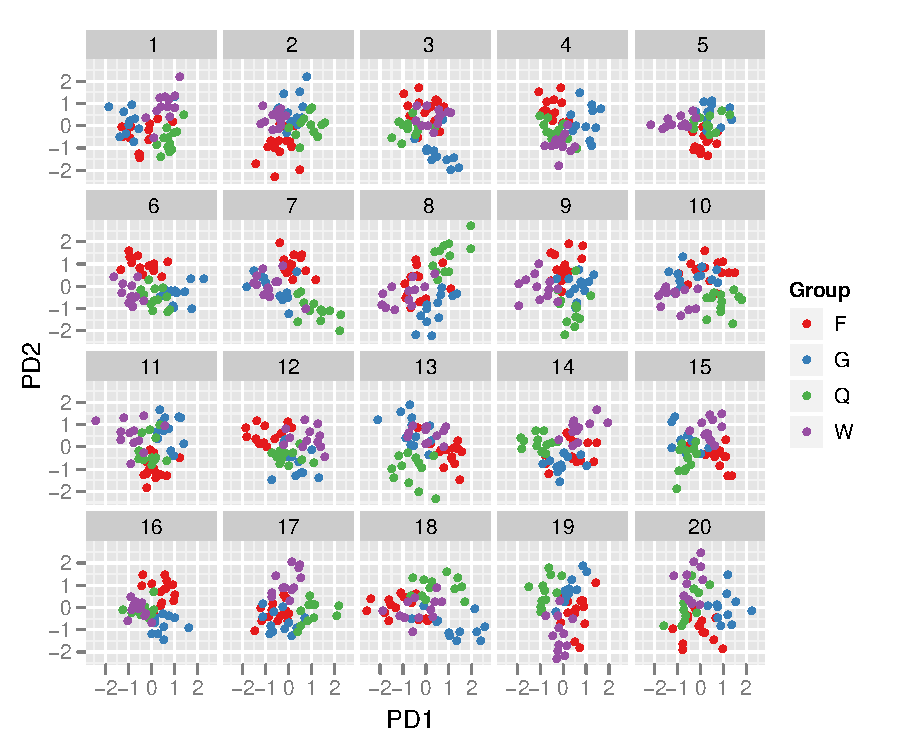
\includegraphics{toth_lineup_pda.pdf}} \end{center}
		\end{column}
	\end{columns}  

\end{frame}



%\begin{frame}
%\frametitle{90\% Confidence Interval}
%\begin{itemize}
%\item We noted the number of dimension when the groups were well separated for both 1D and 2D projections for a fixed sample size $n$.
%\item For example, in the previous plots we pick 34 and 31 respectively for the 1D and 2D projection plots.
%\item We took the 5th and the 95th percentile values.
%\item The 90\% C.I. for 1D projections is (24, 34) and that for the 2D projections is (26, 36).
%\end{itemize}
%\end{frame}

\begin{frame}
\frametitle{Conclusions}
\begin{itemize}
\item We used the visual inference method to check the projection pursuit optimization. It seems ok - originally we felt we could pick the ``true'' data too often - which would have meant the algorithm had problems with ordering of classes.
\item We used the projection pursuit to show that there is {\bf fake} separation among the classes for a large number of dimensions of pure noise for a fixed sample size $n$.
\item We used visual methods to get an estimate the number of dimensions at which the fake classes were well separated in 1D and 2D projections. Next step would be to check these values against what would be expected theoretically.
\end{itemize}
\end{frame}

\begin{frame}
\begin{block}{}
\begin{center} \Large{Chapter 3 --- Where's Waldo: Looking closely at a Lineup} \end{center}
\end{block}
\end{frame}

\begin{frame}
\frametitle{Motivation}
\begin{itemize}
\item In classical hypothesis test, the test statistic is compared with all possible values of the sampling distribution.
\item If the test statistic is extreme, we have evidence to disbelieve the null hypothesis.
\item In visual inference using lineup, for a data plot to be extreme, the human judge should pick it as different from the others.
\end{itemize}
\end{frame}

\begin{frame}
\frametitle{Motivation}
\begin{itemize}
\item A human judge can view a finite number of plots although the distribution of null plots may be infinite.
\item This finite choice of null plots poses a small wrinkle in the lineup protocol.
\item There may be a ``bad" random sample of null plots.
\item This might change your decision about believing or disbelieving the null hypothesis.
\item To avoid this problem, we develop techniques to determine the quality of a lineup.
\end{itemize}
\end{frame}

\begin{frame}
\frametitle{Example}
\begin{itemize}
\item A typical lineup to test the independence of $X$ and $Y$ (left) and the same lineup with a `bad' random sample of null plots (right).
\end{itemize}
\begin{columns}
		\begin{column}{0.52\textwidth}
		\begin{figure}
			 \begin{center} \scalebox{0.4}{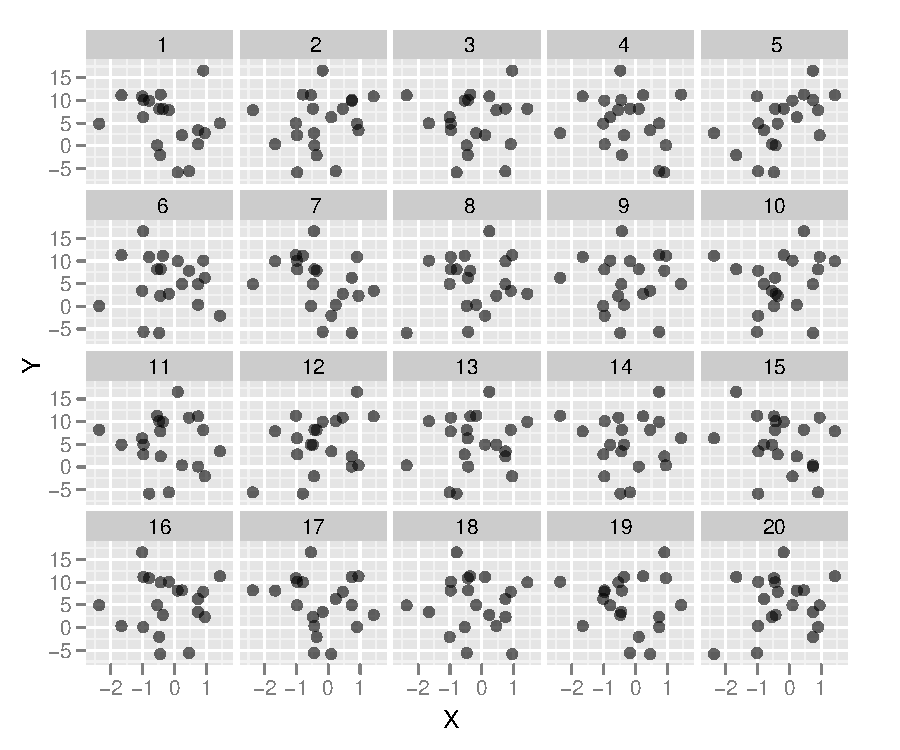
\includegraphics{example-waldo-1.pdf}} 
			% \caption{A typical Lineup.}
			 \end{center}
			 \end{figure}
		\end{column}
		
		\begin{column}{0.52\textwidth}
		\begin{figure}
			 \begin{center} \scalebox{0.4}{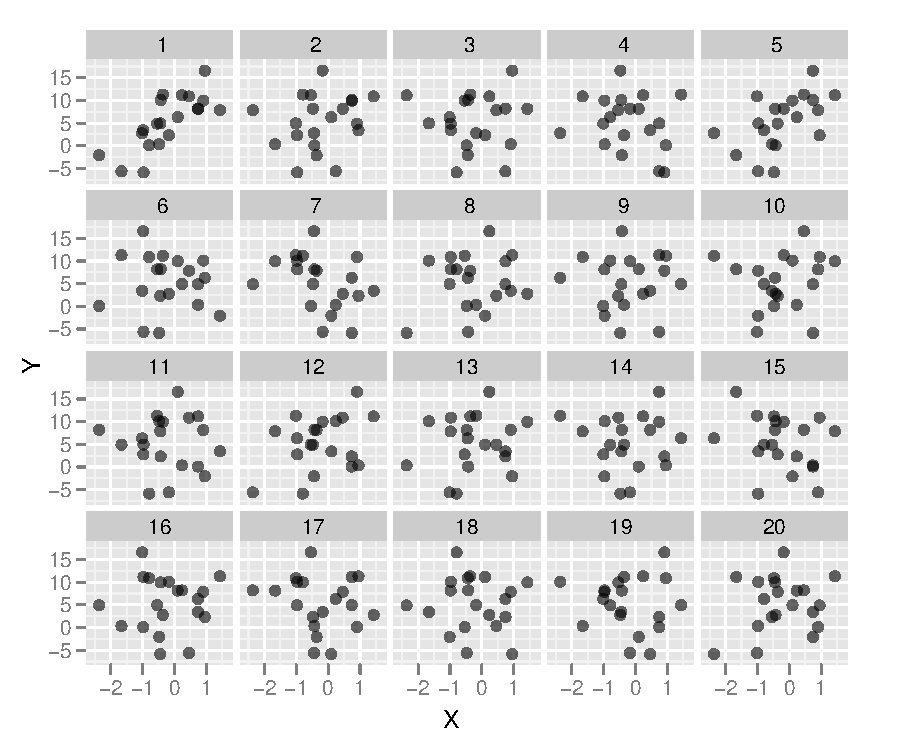
\includegraphics{example-waldo-2.pdf}} 
			%\caption{Lineup with a `bad' sample of null plots.}
			 \end{center}
			 \end{figure}
		\end{column}

\end{columns}
\end{frame}

\begin{frame}
\frametitle{Distance Measures}
\begin{itemize}
\item Different types of distance measures suitable in measuring the distance between the permuted variable and original variable.
\item We used different types so that they can identify the different characteristics.
\item For all distance measures, let $P$ be permutation mapping the set \{$1, 2, \dots,n$ \} onto itself. 
\item Let $[P]$ be a $n \times n$ matrix associated to permutation $P$.
\end{itemize}
\end{frame}

\begin{frame}
\frametitle{1. Hamming Distance}

 The hamming distance $h$ of $P$ is defined as 
\[
h(P) := \sum_{i=1}^n I_{P(i) \neq i},  \text{ where } I_{x} = \left \{ 
\begin{array}{ll}
1 & \text{if } x \text{ is true},\\
0 & \text{otherwise},
\end{array} \right.
\]
i.e. $h(P)$ is a count of the number of fix elements of the function.


\end{frame}


\begin{frame}
\frametitle{2. Euclidean Distance of actual values:}
\begin{itemize}
\item Let $X$ and $Y$ be two continuous variables.
\item Let $Y$ be permuted keeping $X$ fixed. 
\item The Euclidean Distance under permutation is then defined as 
%\red{we need a good short-cut for this distance}
\[
d^2_V(.) := || Y - [P]Y||^2 = \sum_{i=1}^n (Y_i - Y_{P(i)})^2.
\]
\end{itemize}
\end{frame}

\begin{frame}
\frametitle{3. Binned Distance:}
\begin{itemize}
\item $X$ and $Y$ are two continuous variables. 
\item $X$ divided into $p$ bins and $Y$ divided into $q$ bins. 
\item $(i,j)$-th cell represents the $j$-th bin of $Y$ corresponding to the $i$-th bin of $X$. 
\item $(i,j)$-th element of the matrix, $C(X,Y)$ , a $p \times q$ matrix, the number of points falling in the $(i,j)$-th cell, where $i = 1, \dots, p$ , $j = 1, \dots, q$.
\item The Binned distance under permutation is then defined as
\begin{eqnarray*}
b^2_P(.) &:=& ||C(X,Y) - C(X,[P]Y)||^2 \\ &=& \sum_{i=1}^p \sum_{j=1}^q (C_{X_i,Y_j} - C_{X_i,P(Y)_j})^2.
\end{eqnarray*}
\end{itemize}

\end{frame}

\begin{frame}
\frametitle{4. Weighted Bin Distance:}
	\begin{columns}
		\begin{column}{0.52\textwidth}
		\begin{itemize}
\item Using the same setup of the binned distance.
\item The weighted bin distance under permutation is defined as 
\begin{eqnarray*}
& & w_P^2(.)\\ &:=&||W(X,Y) - W(X,[P]Y))||^2 \\ &=& \sum_{i=1}^n (W_{X_{i},Y_i} - W_{X_i,P(Y)_i})^2 , 
\end{eqnarray*}
\item $W_{X_i,Y_i}$ denotes the joint (empirical) density of $X$, $Y$ at location $(X_i, Y_i)$. 
\end{itemize}	
			
		\end{column}
		
		\begin{column}{0.5\textwidth}
			 \begin{center} \scalebox{0.35}{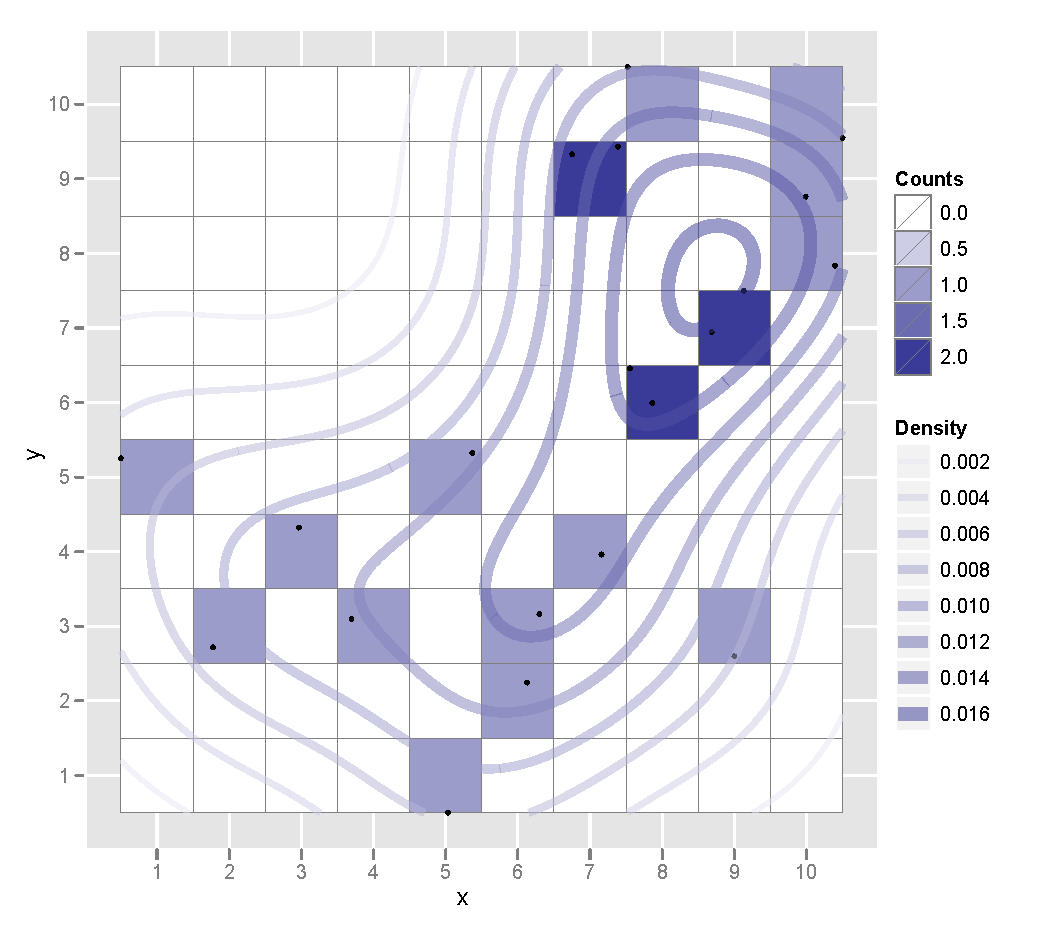
\includegraphics{wbdist.pdf}} \end{center}
		\end{column}
	\end{columns}  
\end{frame}

\begin{frame}
\frametitle{5. $t$ statistic: }
\begin{itemize}
\item We used the test statistic of a t-test based on the correlation coefficient $r$. 
\item  $$t =\frac{r \sqrt{n - 2}}{\sqrt{1 - r^2}}$$ where $n$ is the number of observations in $X$ or $Y$. 
\item This is the only measure that makes a distributional assumption that the ($X$,$Y$) follows approximately a bivariate Normal distribution. 
\item Hence the $t$-statistic follows a t distribution with ($n$ - 2) degrees of freedom.
\end{itemize}
\end{frame}

\begin{frame}
\frametitle{6. Spearman's rank correlation $\rho$ : }
\begin{itemize}
\item $\rho$ is a nonparametric alternative to the correlation coefficient with Kendall's $\tau$. 
\item $X$ and $Y$ are converted into the ranks $x$ and $y$. 
\item Assuming there are no ties in the data, the differences $d_i=x_i - y_i$ between the ranks of each observation between the two variables are calculated 
\item $\rho$ is given as $$\rho = 1 - \frac{6\sum_{i=1}^n d_i^2}{n(n^2 - 1)}$$ 
\item $\rho$ works better than $r$ if the data contains some outliers. 
\item Kendall's $\tau$ is computationally intensive.
\end{itemize}
\end{frame}

\begin{frame}
\frametitle{7. Euclidean Distance of Permutations: (New Work)}

The Euclidean distance of permutations $P$ is 
\[
d^2_P(.) = \sum_{i=1}^n ( i - P(i))^2.
\]
where $i = \{1, 2, ..., n\}$

\end{frame}

\begin{frame}
\frametitle{8. Canberra Distance: (New Work)}
The canberra distance under permutation is defined as
%\begin{eqnarray*}
\[
c^2_P(.)  = \left \{ 
\begin{array}{ll}
\sum_{i=1}^p \sum_{j=1}^q \frac{ |C_{X_i,Y_j} - C_{X_i,P(Y)_j}|}{ C_{X_i,Y_j} + C_{X_i,P(Y)_j}} & \text{if } C_{X_i,Y_j} + C_{X_i,P(Y)_j} > 0,\\
0 & \text{otherwise},
\end{array} \right.
\]

\end{frame}

\begin{frame}
\frametitle{9. Weighted Canberra Distance: (New Work)}
The weighted canberra distance under permutation is defined as 
%\begin{eqnarray*}
\[
wc_P^2(.) = \left \{ 
\begin{array}{ll}
\sum_{i=1}^p \sum_{j=1}^q \frac{ |W_{X_i,Y_j} - W_{X_i,P(Y)_j}|}{ W_{X_i,Y_j} + W_{X_i,P(Y)_j}} & \text{if } W_{X_i,Y_j} + W_{X_i,P(Y)_j} > 0,\\
0 & \text{otherwise},
\end{array} \right.
\] 
%\end{eqnarray*}
where like the weighted bin distance, $W_{X_i,Y_i}$ denotes the joint (empirical) density of $X$, $Y$ at location $(X_i, Y_i)$. 

\end{frame}

\begin{frame}
\frametitle{10. Correlation between $Y$ and $[P]Y$: (New Work)}
\begin{itemize} 
\item The correlation between the $Y$ and $[P]Y$ is defined as
\[
r_P(.) = \frac{ \sum_{i=1}^n (Y_i - \bar{Y_i})(Y_{P(i)} - \bar{Y}_{P(i)})}{\sqrt{\sum_{i=1}^n (Y_i - \bar{Y_i})^2}\sqrt{\sum_{i=1}^n (Y_{P(i)}- \bar{Y}_{P(i)})^2}}.
\]
%\item A high value implies the null plot close to the observed plot.
\end{itemize}
\end{frame}

\begin{frame}
\frametitle{11. Hausdorff Distance: (New Work)}
\begin{itemize}
\item Let $A = \{a_1, a_2, \dots, a_n\}$ and $B = \{b_1, b_2, \dots, b_n\}$ be two finite point sets. 
\item The Hausdorff distance between A and B is defined as
 \[
H_P(.)  = max (h(A, B), h(B, A))
\]
where 
\begin{eqnarray*}
h(A, B) &:=& \max_{a \in A} \min_{b \in B} ||a - b|| \\ & = & \max_{a \in A} \min_{b \in B} \sqrt{\sum_{i=1}^n (a_i - b_i)^2}
\end{eqnarray*}
\item In our case $A$ and $B$ are the points whose coordinates are $(X_i, Y_i)$ and $(X_i, Y_{P(i)})$ respectively. 
\item This measure is computationally intensive.

\end{itemize}

\end{frame}


\begin{frame}
\frametitle{People's Pick}
\begin{itemize}
\item A human subject's experiment was conducted.
\item Each participant was shown 5 lineups.
\item 15 participants were asked which plot exhibited the strongest positive association.
\item Then after revealing the location, they were asked the plot that looked most similar to the observed data plot.
\item Most people provided 2-3 closest.
\item Participants were not requested to order their closeness picks. 
\item We combined the picks as 
\[
\hbox{People's pick} = \frac{2}{3} p_{1,2} + \frac{1}{3} p_{2,3}
\]
\end{itemize}
\end{frame}


\begin{frame}
\frametitle{Example using Scatterplot}
\begin{itemize}
\item Two continuous variables $X$ and $Y$.
\item Interested in whether there exists a significant positive association.
\item Assuming independence, the null plots are generated by permuting $Y$ keeping $X$ fixed.
\item The test statistic, the observed plot is placed randomly among the 19 null plots in a lineup.
\item The distances of all the null plots to the observed plot is computed.
\end{itemize}

\end{frame}

\begin{frame}
\frametitle{Scatterplot Example}
	\begin{columns}

	\begin{column}{0.45\textwidth}
	 \begin{center}
  		\scalebox{0.33}{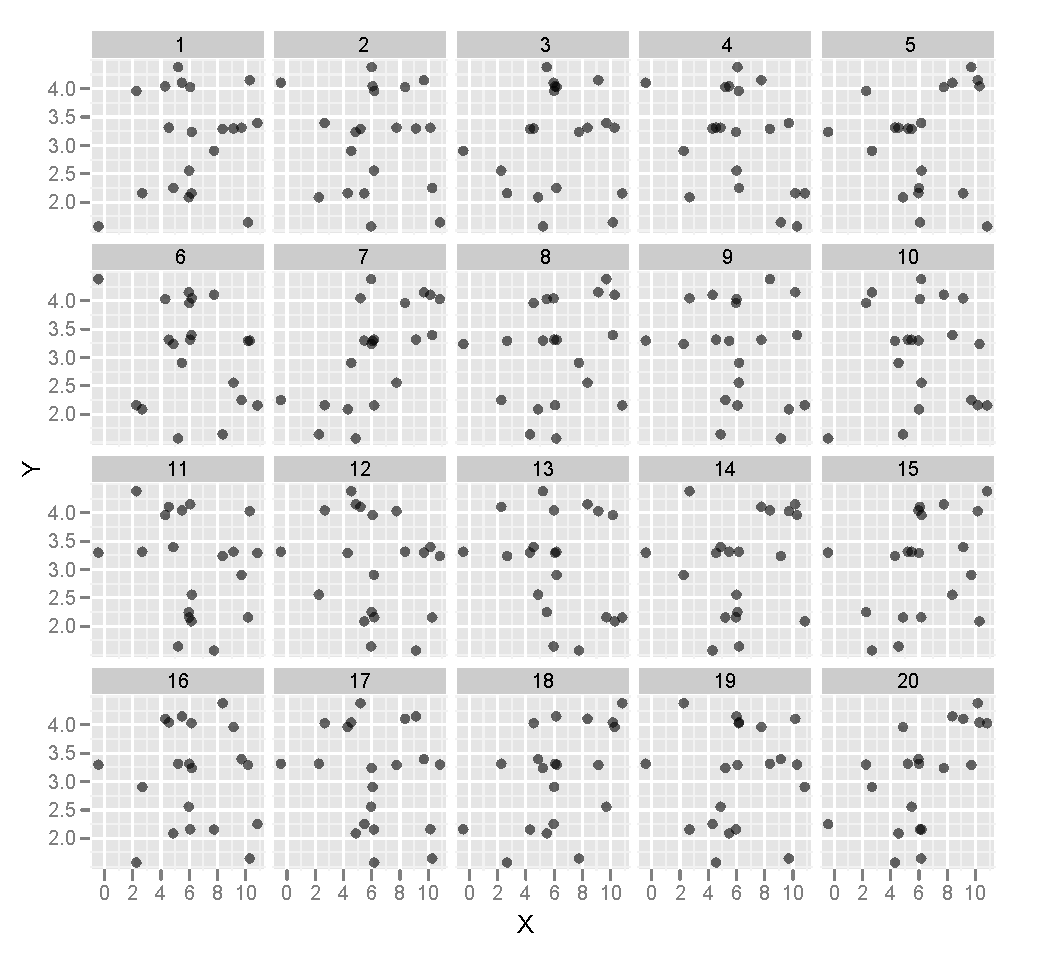
\includegraphics{sca2.pdf}} 
		 \end{center}
	\end{column}

	\begin{column}{0.55\textwidth}
		 \begin{center}
  		\scalebox{0.33}{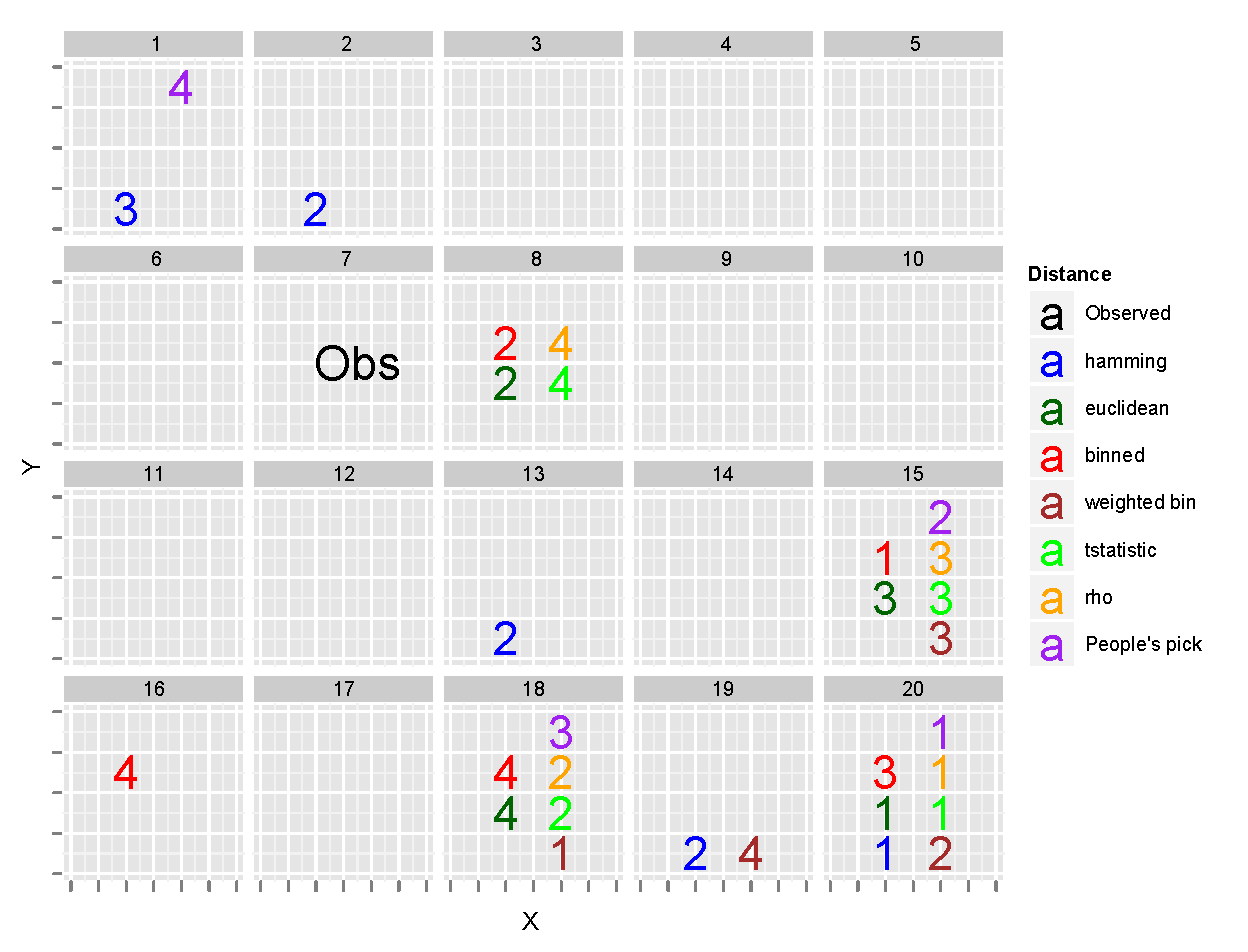
\includegraphics{dist_lineup_final.pdf}} 
		 \end{center}
	\end{column}
\end{columns}
\end{frame}

\begin{frame}
\frametitle{$z$-score}
	\begin{columns}

	\begin{column}{0.55\textwidth}
		\begin{itemize}
		\item We generate empirical distributions based on 10,000 permutations of $Y$.
		\item The `difficulty' of spotting the observed data plot is measured by how far away the red 		line is from the blue lines.
		\item we calculated z-score values by
		$$z_k = \frac{m_k - \mu_m}{\sigma_m}$$
		where $m_k$ is a particular distance measure for the $k$-th plot
		\item  $\mu_m$ and $\sigma_m$ are the mean and the standard deviation of the empirical 		distribution of the measure.
		\end{itemize}
	\end{column}

	\begin{column}{0.45\textwidth}
		 \begin{center}
  		\scalebox{0.33}{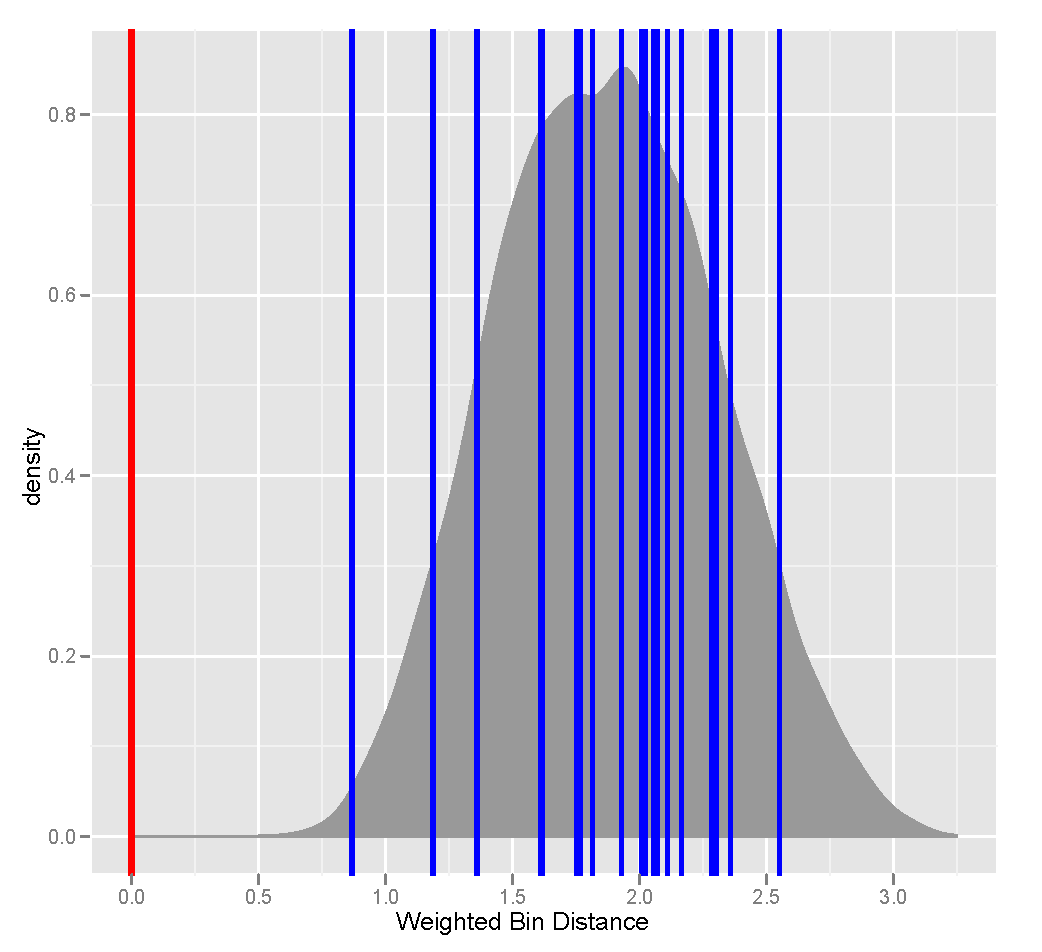
\includegraphics{emp_wbdist3.pdf}} 
		 \end{center}
	\end{column}
\end{columns}
\end{frame}

\begin{frame}
\begin{itemize}
\item We compare the null plots to the observed plot on the basis of the z-scores.
\item Since all of the distance measures are 0 for the observed plot, the z-scores for the observed plot is $- \mu_m/ \sigma_m$.
\item A low z-score indicates that the null plot is close to the observed plot.
\item A high z-score indicates that the null plot is far from the observed plot.
\end{itemize}
\end{frame}

\begin{frame}
\frametitle{Table Showing the $z$-scores and Percentile Values}
\begin{table}[hbt]
	\vspace{-.4in}
%\caption{Percentile values and $z$ scores of closest distances from the observed data plot in the lineup of Figure~\ref{sca_1}. Rows are ordered according to minimal distance from the observed data plot within each of the distance measures. Plot 20 is close to the observed data plot for all  of the distances.}
%Table showing the different distance matrices and the percentile values of each distance 
%\red{also explain the ordering - and don't report the numbers at this precision.} \green{I am not sure what precision I should use.}
%
\centering  % centering table
\begin{tabular}{l r rrrr r rrr}  % creating 10 columns
\hline                       % inserting double-line
Dist. & PlotNo &\multicolumn{4}{c}{$z$-score} & &\multicolumn{3}{c}{Perc. Val} \\ [0.5ex]   
 \cline{1-1}\cline{3-6}\cline{8-10}
 & & H & E & B & W Bin & & t & $\rho$ & P   \\     [0.5ex]
\hline
%% Entering 4th row
H  & 20 & $\bf -2$ & $-1.7$ & $-1.7$ & $-1.6$ & & 0.3 & 0.8 & 45.8 \\[-0.5ex]
 & 2 & $\bf -1$ & 0.3 & $-0.4$ & $-1.0$ & & 62.2 & 38.4 & 0.0\\[-0.5ex]
% & 13 & $\bf  -1$ & 0.3 & 0.7 & 1.1 & & 85.6 & 88.9 & 0.0 \\[-0.5ex]
%& 19 & $\bf -1$ & $0.6$ & $-1.3$ & $-1.2$ &  & $36.8$ & $22.5$ & 0.0 \\[-0.5ex]
% & 1 & $\bf 0$ & $-1.2$ & 0.7 & $-0.6$ & & 22.3 & 33.8 & 8.3 \\[1ex]

%%% Entering 4th row
E  & 20 & $-2$ & $\bf -1.8$ & $-1.7$ & $-1.6$ & & $0.3$ & $0.8$  & 45.8 \\[-0.5ex]
		 & 8 & $ 1$ & $\bf -1.7$ & $-2.2$ & $-1.0$ & & $18.1$ & $10.4$ & 0.0 \\[-0.5ex]
% 		& 15 & $1$ & $\bf -1.7$ & $-2.7$ & $ -1.4$ & & $7.7$ & $4.5$ & 33.3\\[-0.5ex]
% 		& 18 & $1$ & $\bf -1.4$ & $-1.3$ & $ -2.0$ & & $1.9$ & $2.3$ & 12.5\\[1ex]

%%% Entering 4th row
Bin  & 15 & $1$ & $-1.7$ & $\bf -2.7$ & $ -1.4$ & & $7.7$ & $4.5$ & 33.3\\[-0.5ex]
	    & 8 & $ 1$ & $-1.7$ & $\bf -2.2$ & $-1.0$ & & $18.1$ & $10.4$ & 0 \\[-0.5ex]
%	   & 20 & $-2$ & $-1.8$ & $\bf -1.7$ & $ -1.6$ & & $0.3$ & $0.8$ & 45.8 \\[-0.5ex]
% 		& 16  & $1$ & $-0.9$ & $\bf -1.3$ & $-0.2$ & & 55.1 & 56.1 & 0\\[-0.5ex]
%		& 18 & $1$ & $-1.4$ & $\bf -1.3$ & $\bf -2.0$ & & $1.9$ & $2.3$ & 12.5\\[1ex]
%
%%% Entering 4th row
W Bin & 18 & $1$ & $-1.4$ & $-1.3$ & $\bf -2.0$ & & $1.9$ & $2.3$ & 12.5 \\[-0.5ex]
		 & 20 & $-2$ & $-1.8$ & $-1.7$ & $\bf -1.6$ & & $0.3$ & $0.8$ & 45.8 \\[-0.5ex]
% 		& 15 & $1$ & $-1.7$ & $-2.7$ & $\bf -1.4$ & & $7.7$ & $4.5$ & 33.3 \\[-0.5ex]
% 		& 19 & $-1$ & $0.6$ & $-1.3$ & $\bf -1.2$ & & $36.8$ & $22.5$ & 0\\[1ex]

%%% Entering 4th row
t   & 20 & $-2$ & $-1.8$ & $-1.7$ & $ -1.6$ & & $\bf 0.3$ & $0.8$ & 45.8 \\[-0.5ex]
		  & 18 & $1$ & $-1.4$ & $-1.3$ & $ -2.0$ & & $\bf 1.9$ & $2.3$ & 12.5\\[-0.5ex]
%		& 15 & $1$ & $-1.7$ & $-2.7$ & $ -1.4$ & & $\bf 7.7$ & $4.5$ & 33.3 \\[-0.5ex]
% 		 & 8 & $ 1$ & $-1.7$ & $-2.2$ & $-1.0$ & & $\bf18.1$ & $10.4$ & 0 \\[1ex]

%%% Entering 4th row
 $\rho$  & 20 & $-2$ & $-1.8$ & $-1.7$ & $ -1.6$ & & $0.3$ & $\bf 0.8$ & 45.8 \\[-0.5ex]
		   & 18 & $1$ & $-1.4$ & $-1.3$ & $ -2.0$ & & $1.9$ & $\bf 2.3$ & 12.5 \\[-0.5ex]
%		 & 15 & $1$ & $-1.7$ & $-2.7$ & $ -1.4$ & & $7.7$ & $\bf 4.5$ & 33.3 \\[-0.5ex]
% 		 & 8 & $ 1$ & $-1.7$ & $-2.2$ & $-1.0$ & & $18.1$ & $\bf 10.4$ & 0\\[1ex]

People's  	& 20 & $-2$ & $-1.8$ & $-1.7$ & $ -1.6$ & & $0.3$ & $0.8$ & $\bf 45.8$ \\[-0.5ex]  
		 & 15 & $1$ & $-1.7$ & $-2.7$ & $ -1.4$ & & $7.7$ & $4.5$ & $\bf 33.3$ \\[-0.5ex]
%		  & 18 & $1$ & $-1.4$ & $-1.3$ & $ -2.0$ & & $1.9$ & $2.3$ & $\bf 12.5$ \\[1ex]

\hline
Actual & 7  & $-19$ & $-8.5$ & $-9.9$ & $-4.1$ & & 0.1 & 0.2 & 93.3\\[1ex]
\hline
\end{tabular}
\label{sca_table}
\end{table}

\end{frame}


\begin{frame}
\frametitle{Results}
\begin{itemize}
\item We plot the People's pick against the $z$-scores and the percentile values.
\item $R^2$ gives a measure of the correlation between People's pick and the distance measures.
\item Median $R^2$ indicates that Spearman's $\rho$ works best followed by $t$-statistic and weighted bin.
\end{itemize}
\end{frame}

%\begin{frame}
%\begin{figure}[htbp]
%\centering
%\subfigure[]{
%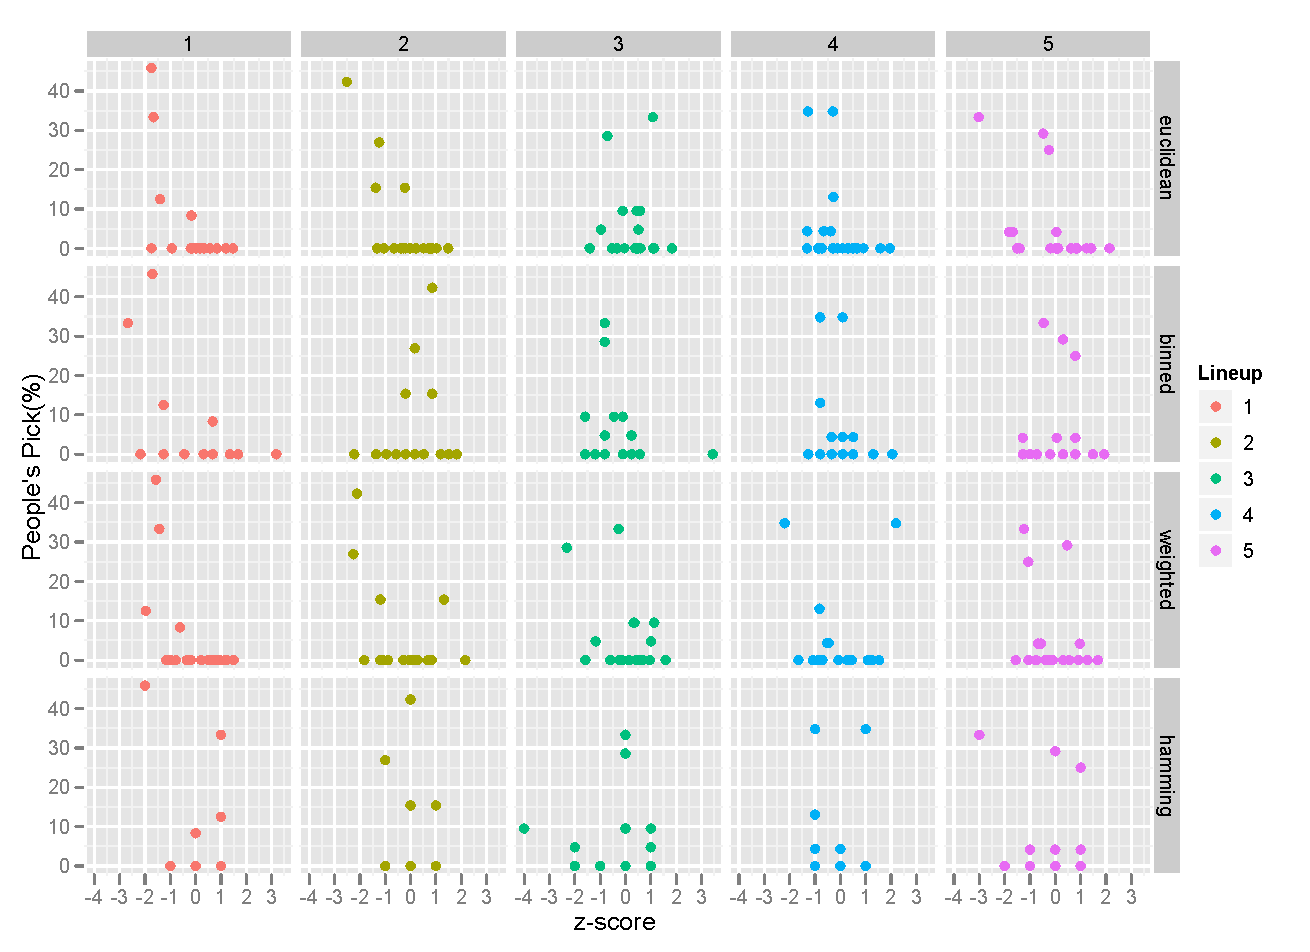
\includegraphics[scale=0.27]{dist_vs_zscore.pdf}
%\label{dist_1}
%}
%\subfigure[]{
%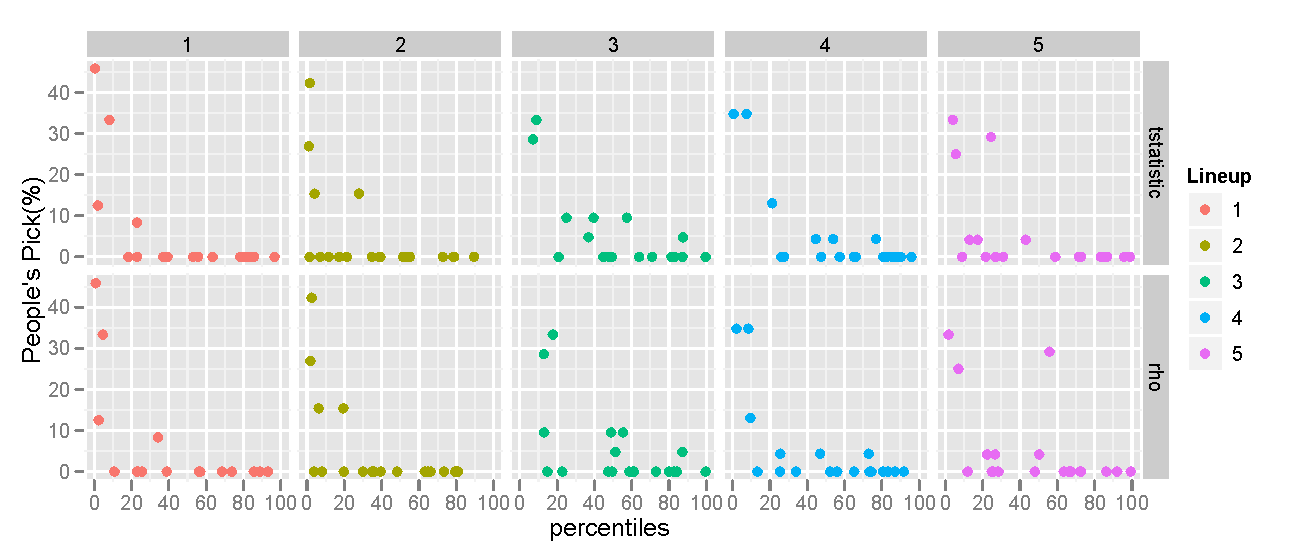
\includegraphics[scale=0.27]{dist_vs_percentile.pdf}
%\label{dist_2}
%}
%\label{dist_z_perc}
%	\vspace{-.1in}
%%\caption[Optional caption for list of figures]{(a) Scatterplot of the People's pick against the z-scores for each distance measure colored by the lineups. (b) Scatterplot of the People's pick against the percentiles for t-statistic and Spearman's $\rho$ colored by the lineups. }
%%{Caption of subfigures \subref{fig:subfig1}, \subref{fig:subfig2} and \subref{fig:subfig3}}
%\end{figure}
%\end{frame}

\begin{frame}
\begin{figure}[htbp]
\centering
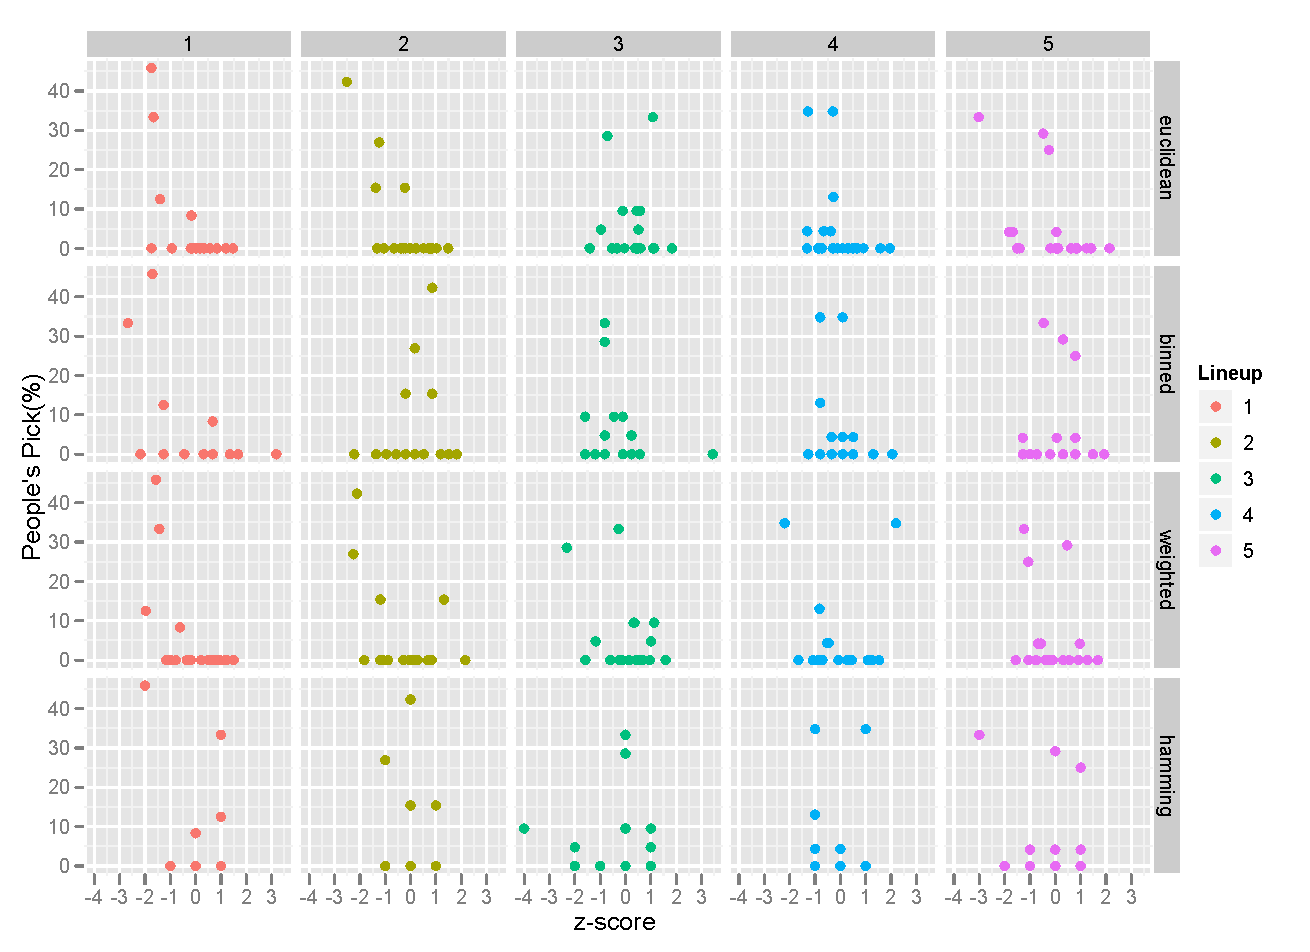
\includegraphics[scale=0.45]{dist_vs_zscore.pdf}
\caption{Scatterplot of the People's pick against the z-scores for each distance measure colored by the lineups. }
%{Caption of subfigures \subref{fig:subfig1}, \subref{fig:subfig2} and \subref{fig:subfig3}}
\end{figure}


\end{frame}

\begin{frame}
\begin{figure}[htbp]
\centering
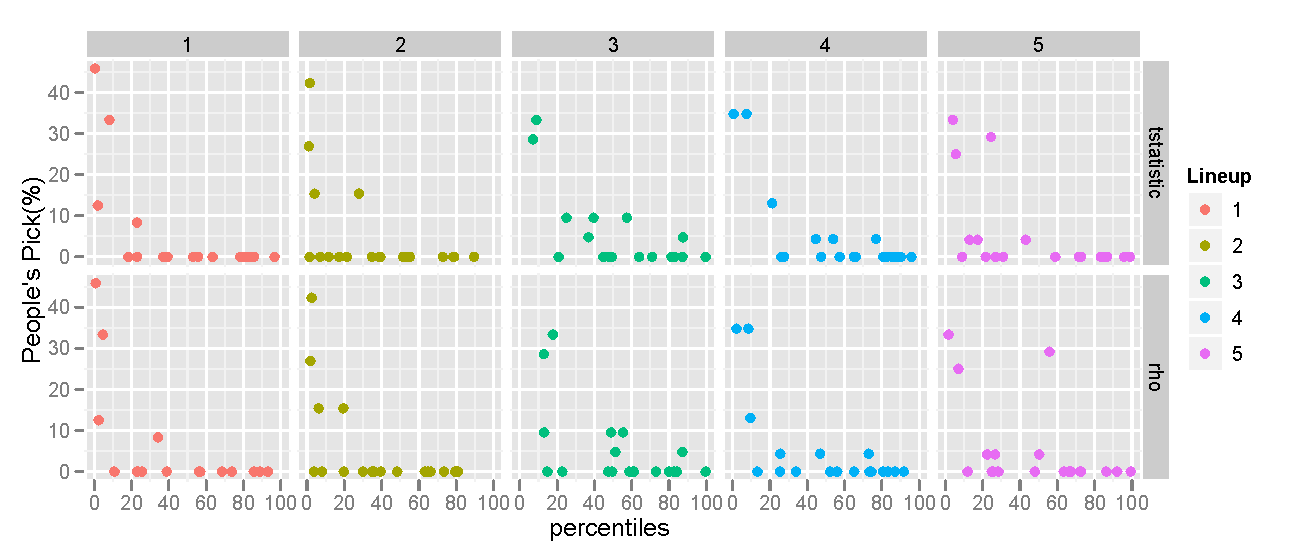
\includegraphics[scale=0.45]{dist_vs_percentile.pdf}
\caption{Scatterplot of the People's pick against the percentiles for t-statistic and Spearman's $\rho$ colored by the lineups. }
%{Caption of subfigures \subref{fig:subfig1}, \subref{fig:subfig2} and \subref{fig:subfig3}}
\end{figure}


\end{frame}

\begin{frame}
\frametitle{Recent Developments}
	\begin{columns}

	\begin{column}{0.55\textwidth}
		\begin{itemize}
		\item We generate `null datasets' based on 10,000 permutations of $Y$.
		\item Calculate the distance measures between the actual data and each of these `null datasets'. 
		\item Select those datasets which are closest to the observed data according to each of  the distance measures.
		\item Plot the observed data with these sets of null data in a plot-matrix.
		\item A human judge has to pick which is the closest to the actual plot.
		\end{itemize}
	\end{column}

	\begin{column}{0.45\textwidth}
		 \begin{center}
  		\scalebox{0.38}{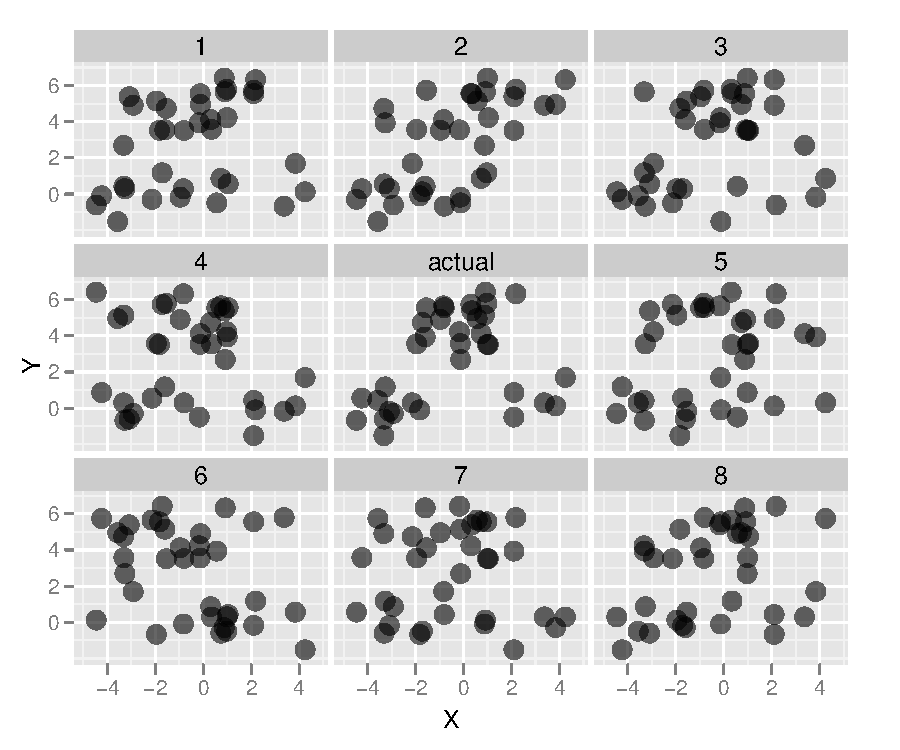
\includegraphics{minimum.pdf}} 
		 \end{center}
	\end{column}
\end{columns}
\end{frame}



\begin{frame}
\frametitle{Future Work}
\begin{itemize}
\item Design an experiment to find the distance measure which is closest to the visual distance.
\item Look at more general relationships between $X$ and $Y$. 
\end{itemize}
\end{frame}


\begin{frame}
\frametitle{Plans and Timeline}
%\vspace{-1cm}
\begin{table}[hbtp]
\small
%\caption{Jobs completed so far}
\centering 
\begin{tabular}{|p{3cm}|p{6cm}|l|} 
\hline
Task &  Description & Status date\\ %[0.5ex] % inserts table %heading 
\hline
Chapter 2: Large $p$, small $n$ (Paper)  & A comparison was done between data with real separation and data with no real separation to examine the performance of projection pursuit in \texttt{tourr} package. Published in proceedings of the ASA. & Jan 2011 \\
(Poster) & Poster presented in the 4th Annual Midwest Statistics Research Colloquium. & Mar 2011 \\
(Pilot Study) & First pilot study to examine the performance of projection pursuit.   & May 2011\\ 
%Turk Experiment & The first Amazon Mechanical Turk experiment for obtaining the power of visual inference described in chapter 2. Our web site is used to collect data from the participants recruited from Amazon Mechanical Turk \vspace{.1in} & Nov 2010 \\
(Talk) & Presented the results of Chapter 2 in Joint Statistical Meetings, Miami Florida  & July 2011 \\
(Journal Article) & Expand paper based on example of LDA on expression data  & {\bf Oct 2012} \\\hline
\end{tabular}
\label{tbl:tjob}
\end{table}	
\end{frame}

\begin{frame}
%\frametitle{Plans and timeline}
\vspace{-0.5cm}
\begin{table}[hbtp]
\small
%\caption{Jobs completed so far}
\centering 
\begin{tabular}{|p{2.5cm}|p{6cm}|l|} 
\hline
Task &  Description & Status date\\ %[0.5ex] % inserts table %heading 
\hline
Chapter 3: Lineup Metrics (Paper) & The paper titled ``Where's Waldo: Looking Closely at a Lineup'' submitted to ASA and won student paper award 2012. Available as a department tech report.  & Dec 2011 \\
(New Work) & Comparing distance metrics with visual selections, several new distance metrics defined and examined. & {\bf April-Sep 2012}\\
(Talk) & Present the paper that won the ASA student paper award 2012 in JSM  & {\bf Aug 2012}\\
(Turk Experiment) & The first turk experiment to examine which distance measure among a selected set is most similar to the visual distance  & {\bf Sep 2012} \\
(R Package)  & Expand the R package, {\tt nullabor} to include lineup metrics of the quality of a lineup. & {\bf Nov 2012}\\
(Journal Article) & Refine the JSM paper into a journal article with the new metrics and results of the Turk study. & {\bf Dec 2012}\\ \hline
\end{tabular}
\label{tbl:tjob}
\end{table}

\end{frame}

\begin{frame}
\vspace{-0.5cm}
\begin{table}[hbtp]
\small
%\caption{Jobs completed so far}
\centering 
\begin{tabular}{|p{2.5cm}|p{6cm}|l|} 
\hline
Task &  Description & Status date\\ %[0.5ex] % inserts table %heading 
\hline
Chapter 4: Teaching Material & Developed a first draft of lecture notes (slides), worksheet and quizzes, to use visual inference to explain hypothesis testing. Tested this with Statistics 226, and also Statistics 101 & Mar-Apr 2012 \\
 & Refine the lecture notes, worksheets and quizzes, and use during the summer session of Stat 226. & {\bf July 2012} \\
 (Human subjects experiment) & Request IRB approval to conduct an experiment to compare understanding of hypothesis testing between students exposed to visual inference explanation and traditional teaching methods. & {\bf Aug 2012} \\
(R Package)  & Expand the R package {\tt nullabor-teaching} to incorporate games for undergraduates utilizing visual inference and the lineup metrics. & {\bf Aug-Nov 2012} \\
(Journal Article) & Publish the teaching material and results of human subjects experiment. & {\bf Mar 2013}\\\hline
%Paper & Paper based on the real data analysis and implementation of visual inference technique with medical data from summer internship with Novartis \vspace{.1in} & May 2012\\
%\hline 
\end{tabular}
\label{tbl:tjob}
\end{table}
\end{frame}

\begin{frame}
\begin{table}[hbtp]
\small
%\caption{Jobs completed so far}
\centering 
\begin{tabular}{|p{2.5cm}|p{5cm}|l|} 
\hline
Task &  Description & Status date\\ %[0.5ex] % inserts table %heading 
\hline
Chapter 5: Application & Apply lineups to discovery of structure in the GE data. We expect that this will lead to another journal article. & {\bf Dec 2012-Mar 2013}\\ \hline
Thesis defense & Defend my thesis and graduate & {\bf May 2013}\\
\hline 
\end{tabular}
\label{tbl:tjob}
\end{table}
\end{frame}
%\begin{frame}
%\frametitle{Conclusion}
%\begin{itemize}
%\item We take a closer look at the null plots in a lineup.
%\item We do that with the help of some distance measure that gives a measure of closeness of the null plots to the observed plot.
%\end{itemize}
%\end{frame}

\end{document}
%\begin{frame}
%  \frametitle{Comparison: Visual vs Mathematical Inference}
%  Model: $Y = \beta_0 + \beta X + \epsilon $; $\epsilon \stackrel{iid}{\sim} N(0,\sigma^2)$ 
%  {\small
%  \begin{table}[ht] 
%		\begin{tabular}{llll} 
%			\hline
%				   & Mathematical Inference &  Visual Inference \\ %[0.5ex] % inserts table %heading 
%			\hline
%				  Hypothesis & $H_0: \beta=0$ vs $H_1: \beta \ne 0$& $H_0: \beta=0$ vs $H_1: \beta \ne 0$\\
%
%				 & \begin{minipage}[h]{1cm} \begin{center} \scalebox{0.18}{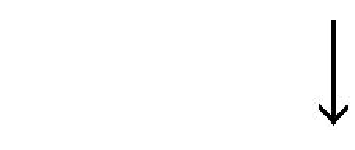
\includegraphics{down_arrow.pdf}} \end{center} \end{minipage} & \begin{minipage}[h]{1cm} \begin{center} \scalebox{0.18}{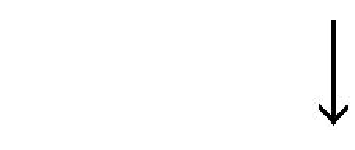
\includegraphics{down_arrow.pdf}} \end{center} \end{minipage} \\
%				  
%				 Test statistic & $T(y)=\frac{\hat{\beta}}{se(\hat{\beta})}$ & $T(y)=$ \begin{minipage}[h]{1cm} \begin{center} \scalebox{0.08}{\includegraphics{stat_intercept.pdf}} \end{center} \end{minipage} \\
%				 
%				 & \begin{minipage}[h]{1cm} \begin{center} \scalebox{0.18}{\includegraphics{down_arrow.pdf}} \end{center} \end{minipage} & \begin{minipage}[h]{1cm} \begin{center} \scalebox{0.18}{\includegraphics{down_arrow.pdf}} \end{center} \end{minipage} \\
%				 
%				 Null Distribution & $f_{T(y)}(t); $\begin{minipage}[h]{1cm} \begin{center} \scalebox{0.08}{\includegraphics{stat_mathematical_test.pdf}} \end{center} \end{minipage} & $f_{T(y)}(t); $ \begin{minipage}[h]{1cm} \begin{center} \scalebox{0.08}{\includegraphics{test_slope.pdf}} \end{center} \end{minipage} \\
%
%				 & \begin{minipage}[h]{1cm} \begin{center} \scalebox{0.18}{\includegraphics{down_arrow.pdf}} \end{center} \end{minipage} & \begin{minipage}[h]{1cm} \begin{center} \scalebox{0.18}{\includegraphics{down_arrow.pdf}} \end{center} \end{minipage} \\
%				 
%				 
%				 Reject $H_0$ if & observed $T$ is extreme & observed plot is identifiable \\
%			\hline 
%		\end{tabular}
%	\end{table}	
%	}
%\end{frame} 
%
%
%
%
%\begin{frame}
%\frametitle{$Y_i = \beta_0 + \beta_1 X_{i1} + \beta_2 X_{i2}+ \beta_3 X_{i1} X_{i2}+ ... + \epsilon_i $ ; $\epsilon_i \stackrel{iid}{\sim} N(0,\sigma^2)$}
%
%{\footnotesize
%\begin{table}[ht] 
%	\centering 
%		%\begin{tabular}{m{3cm}m{2.5cm}m{2.6cm}m{5.5cm}} 
%		\begin{tabular}{lll} 
%			\hline
%				Null Hypothesis & Type &  Test Statistic   \\ %[0.5ex] % inserts table %heading 
%			\hline 
%								$H_0: \beta_k=0$ & Residual Plot & \begin{minipage}[h]{1cm}\begin{center}  	\scalebox{0.081}{\includegraphics{stat_bet_p.pdf}} \end{center} \end{minipage}  \\ 
%				
%				$H_0: X$ Linear & Residual Plot & \begin{minipage}[h]{1cm}\begin{center}   \scalebox{0.081}{\includegraphics{stat_nonlinear.pdf}} \end{center} \end{minipage} \\ 
%
%				\begin{minipage}[h]{4cm} $H_0: \beta_k=0$ for categorical $X_k$ \end{minipage} & Boxplot & \begin{minipage}[h]{1cm}\begin{center}  \scalebox{0.13}{\includegraphics{stat_category.pdf}} \end{center} \end{minipage}  \\ 
%								
%				\begin{minipage}[h]{4cm} $H_0: \beta_k=0$ (interaction 
%with categorical $X_k$) \end{minipage} & Scatter plot & \begin{minipage}[h]{1cm}\begin{center} \scalebox{0.081}{\includegraphics{stat_interection.pdf}} \end{center} \end{minipage}\\				
%
%				$H_0:$ Model Fits & Histogram & \begin{minipage}[h]{1cm}\begin{center}  \scalebox{0.081}{\includegraphics{stat_goodness_simple.pdf}} \end{center} \end{minipage} \\[.5ex] % [1ex] adds vertical space 
%			\hline 
%		\end{tabular} 
%	\label{tbl:stat_simple} 
%\end{table} 		
%}
%\end{frame}
%
%
%\begin{frame}
%  \frametitle{$Y = \beta_0 + \beta_1 X_{1} + \beta_2 X_{2}+ \beta_3 X_{1} X_{2}+  \epsilon $ ; $\epsilon \sim N(0,\sigma^2)$}
%	\begin{columns}
%		\begin{column}{0.4\textwidth}
%		  \begin{itemize}
%			  \item $H_0: \beta_3=0$
%			  \item Can you identify the plot of observed data? 
%		  \end{itemize}		
%			
%		\end{column}
%		
%		\begin{column}{0.6\textwidth}
%			 \begin{center} \scalebox{0.43}{\includegraphics{test_interaction.pdf}} \end{center}
%		\end{column}
%	\end{columns}  
%\end{frame} 
%
%\begin{frame}
%  \frametitle{$Y = \beta_0 + \beta_1 X_{1} + \beta_2 X_{2}+ \beta_3 X_{1} X_{2}+  \epsilon $ ; $\epsilon \sim N(0,\sigma^2)$}
%	\begin{columns}
%		\begin{column}{0.4\textwidth}
%		  \begin{itemize}
%			  \item $H_0: \beta_3=0$
%			  \item Can you identify the plot of observed data? 
%		  \end{itemize}		
%			
%		\end{column}
%		
%		\begin{column}{0.6\textwidth}
%			 \begin{center} \scalebox{0.43}{\includegraphics{test_interaction1.pdf}} \end{center}
%		\end{column}
%	\end{columns}  
%\end{frame} 
%
%\begin{frame}
%  \frametitle{P value and Type-I error}
%	For a lineup of $m$ plots
%	\begin{enumerate}
%	\item p-value for an Individual evaluation
%		\begin{itemize}
%			\item when reject report p-value $\le \frac1m$ .
%			\item when cannot reject report p-value $\ge 1-\frac1m$ .
%		\end{itemize}
%	\item p-value for $N$ independent evaluations
%		\begin{itemize}
%		  \item under Null hypothesis, $Pr$(Reject)=$\frac1m$ for each evaluation.
%			\item number of success $ U \sim Binom(N,\frac1m)$.
%			\item p-value= $Pr(U \ge u)= \sum_{k \ge u}^N {{N \choose k} (\frac1m)^k(1-\frac1m)^{(N-k)}}$ where $u$ be the observed number of success.
%			\item exact probability for discrete variable makes it conservative.
%			\item when $N=1$ this p-value matches with individual judgment p-value
%		\end{itemize}
%	\item type-I error probability = $\frac1m$.
%	\end{enumerate}
%\end{frame}
%
%
%
%
%\begin{frame}
%  \frametitle{Power for testing $H_0: \theta \in \Theta_0$ vs $H_1: \theta \in \Theta^c_0$}
%  \begin{itemize}
%    \item For a lineup of $m$ plots, power function of $\theta$ be defined as 
%    \begin{equation*}
%      \beta(\theta)= 
%        \begin{cases} 
%              \text{Type-I error}=\frac1m & \text{if $\theta \in \Theta_0$,} \\
%              Pr(\text{Reject } H_0) &\text{if $\theta \in \Theta^c_0$.}
%        \end{cases}
%    \end{equation*}
%    \item Estimated power = $\frac uN$ \\
%             $u$ = number of successful evaluations \\
%             $N$ = number of independent evaluations. 
%    \item A generalized mixed linear model can be used to estimate power. 
%  \end{itemize}
%
%\end{frame}
%
%
%\begin{frame}
%  \frametitle{Simulation based experiment}
%  \begin{itemize}
%    \item Model: $Y = \beta_0 + \beta_1 X_1 + \beta_2 X_2 + \epsilon $; $\epsilon \stackrel{iid}{\sim} N(0,\sigma^2)$; $X_2$ categorical
%    \item Hypothesis $H_0: \beta_2=0$ vs $H_1: \beta_2 \ne 0$
%    \item Test statistic is the boxplot of residuals of fitted null model grouped by $X_2$. For lineup plot we simulate data from $N(0,\hat{\sigma}^2)$
%  \end{itemize}
%  \begin{center} \scalebox{0.25}{\includegraphics{stat_category.pdf}} \end{center}
%\end{frame}
%
%
%\begin{frame}
%  \frametitle{Procedure for the experiment}
%    Flow of the experiment
%      \begin{itemize}
%        \item simulate data from the linear model for specific parameters and call it observed data.
%        \item fit null model to the observed data and obtain parameter estimates.
%        \item obtain lineup plot for that specific parameter settings.
%        \item present the lineup plot to individual people to see if they can identify the observed plot.
%      \end{itemize}
%\end{frame}
%
%
%\begin{frame}
%  \frametitle{Survey Setting}      
%      \begin{itemize}    
%        \item Values of parameters considered for survey experiment.
%\begin{table}[hbtp]
%%\caption{Values of parameters considered for survey experiment} % title name of the table
%\centering
%\begin{tabular}{c c r r r r r }
%\hline
%Sample size ($n$) & $\sigma$ &\multicolumn{5}{c}{values for $\beta_2$}
%\\ [0.5ex]
%\hline
%&  5 & 0 & 1 & 3 & 5 & 8  \\[-1ex]
%\raisebox{1.5ex}{100} &12
%& 1 & 3 & 8 & 10 & 16  \\[1ex]
%&  5 & 0 & 1 & 2 & 3 & 5  \\[-1ex]
%\raisebox{1.5ex}{300} & 12
%& 1 & 3 & 5 & 7 & 10  \\[1ex]
%\hline
%\end{tabular}
%\label{tbl:expeiment_params}
%\end{table} 
%        \item For each of the above combinations 3 independent lineup plots were generated.
%        \item Recruited 324 participants through Amazon Mechanical Turk web site. 
%      \end{itemize}    
%\end{frame}
%
%\begin{frame}
%  \frametitle{Expected power}
%        \begin{itemize}
%             \item Under $H_1$ distribution of p-value $p_m$ is right skewed
%             \item Under $H_0$ $p_m \sim $ Uniform(0,1)
%             \item $p_0 = min(p_m) \sim beta(1,m-1)$
%             \item Expected power = $Pr(p_{obs} < p_0)$
%        \end{itemize}	
%			 \begin{center} \scalebox{0.45}{\includegraphics{power_expected.pdf}} \end{center}
%\end{frame} 
%
%\begin{frame}[containsverbatim]
%  \frametitle{Demonstration of data collection from web}
%  \begin{verbatim}
%    http://www.public.iastate.edu/~mahbub/feedback
%  \end{verbatim}
%\end{frame}
%
%\begin{frame}
%\begin{center} \Large{Amazon Turk experiment} \end{center}
%\end{frame}
%
%
%
%\begin{frame}
%  \frametitle{Survey results}
%	\begin{columns}
%		\begin{column}{0.45\textwidth}
%		  \begin{itemize}
%			  \item Sample size 100, $\beta=1$ and $\sigma=5$.
%			  \item For observed plot, p-value is 0.75
%			  \item Most of the responses are 18. Has p-value 0.028 which is minimum. 
%			  \item Attempted 18 times with 5.5\% success.
%		  \end{itemize}		
%			
%		\end{column}
%		
%		\begin{column}{0.55\textwidth}
%			 \begin{center} \scalebox{0.4}{\includegraphics{plot_100_1_5_3.pdf}} \end{center}
%		\end{column}
%	\end{columns}  
%\end{frame} 
%
%
%\begin{frame}
%  \frametitle{Survey results}
%	\begin{columns}
%		\begin{column}{0.45\textwidth}
%		  \begin{itemize}
%			  \item Sample size 300, $\beta=5$ and $\sigma=5$.
%			  \item For observed plot, p-value $ < 0.0001$
%			  \item Attempted 23 times with 100\% success.
%		  \end{itemize}		
%			
%		\end{column}
%		
%		\begin{column}{0.55\textwidth}
%			 \begin{center} \scalebox{0.4}{\includegraphics{plot_300_5_5_1.pdf}} \end{center}
%		\end{column}
%	\end{columns}  
%\end{frame} 
%
%
%\begin{frame}
%  \frametitle{Observed power}
%  \begin{center}  	\scalebox{0.5}{\includegraphics{power_observed.pdf}} \end{center}
%\end{frame}
%
%\begin{frame}
%  \frametitle{Power estimated from logistic model}
%  Sample size = 100, standard deviation = 12
%  \begin{center}  	\scalebox{0.5}{\includegraphics{power_model.pdf}} \end{center}
%\end{frame}
%
%\begin{frame}
%  \frametitle{Power estimated from generalized mixed model}
%  Sample size = 100, standard deviation = 12
%  \begin{center}  	\scalebox{0.55}{\includegraphics{power_subject.pdf}} \end{center}
%\end{frame}
%
%
%\begin{frame}
%\begin{center} \Large{Analysis of experimental data} \end{center}
%\end{frame}
%
%\begin{frame}
%  \frametitle{p-value vs percent correct}
%	\begin{columns}
%		\begin{column}{0.45\textwidth}
%		  \begin{itemize}
%			  \item Percent correct is high with low p-value
%			  \item Can we assume that viewer picks the plot with lowest p-value?
%		  \end{itemize}		
%			
%		\end{column}
%		
%		\begin{column}{0.55\textwidth}
%			 \begin{center} \scalebox{0.4}{\includegraphics{p_value_percent_correct.pdf}} \end{center}
%		\end{column}
%	\end{columns}  
%\end{frame} 
%
%
%\begin{frame}
%  \frametitle{Distribution of time taken}
%	\begin{columns}
%		\begin{column}{0.45\textwidth}
%		  \begin{itemize}
%			  \item Does the distribution differ for male or female?
%			  \item These issues will be examined with other turk experiment results.
%		  \end{itemize}		
%			
%		\end{column}
%		
%		\begin{column}{0.55\textwidth}
%			 \begin{center} \scalebox{0.4}{\includegraphics{dist_time_taken.pdf}} \end{center}
%		\end{column}
%	\end{columns}  
%\end{frame} 
%
%
%\begin{frame}
%  \frametitle{Time taken vs p-value}
%	\begin{columns}
%		\begin{column}{0.45\textwidth}
%		  \begin{itemize}
%			  \item time taken increases over p-value
%			  \item at p-value about 0.01 time taken levels off.
%		  \end{itemize}		
%			
%		\end{column}
%		
%		\begin{column}{0.55\textwidth}
%			 \begin{center} \scalebox{0.4}{\includegraphics{p_value_time.pdf}} \end{center}
%		\end{column}
%	\end{columns}  
%\end{frame} 
%
%\begin{frame}
%  \frametitle{Other considerations}
%  \begin{itemize}
%    \item Visual inference is not the competitor to traditional inference.
%    \item May use where traditional tests can't be used.
%  \end{itemize}
%      
%  \begin{itemize}
%    \item What if not normal?
%      \begin{itemize}
%        \item Extend this study for generalized linear model.
%      \end{itemize}
%    \item Conduct survey   
%      \begin{itemize}
%        \item Examine the other test statistics.
%        \item Assess the sensitivity of power to modeling conditions.
%        \item Discover the most effective specification of a plot.
%      \end{itemize}    
%  \end{itemize}
%\end{frame}
%
%
%\begin{frame}
%\begin{center} \Large{Plans} \end{center}
%\end{frame}
%
%\begin{frame}
%\frametitle{Overview of the completed tasks}
%  \begin{itemize}
%   \item Developed web site for MT experiment
%    \item Visual Inference for regression parameters
%		  \begin{itemize}
%			  \item Introduced method to test hypothesis
%			  \item Proposed methods obtaining power of the test
%			  \item Conducted couple of simulation experiments
%		  \end{itemize}
%    \item Experimental results got attention of people
%		  \begin{itemize}
%			  \item Obtained best poster award
%			  \item Secured ASA student paper award 2011
%		  \end{itemize}	  	  		  		  		  
%  \end{itemize}		  
%\end{frame}
%
%
%
%\begin{frame}
%\frametitle{Overview of the deliverable works}
%  \begin{itemize}
%    \item Amazon Mechanical Turk Experiment
%		  \begin{itemize}
%			  \item Experimental Design
%			  \item How to conduct a experiment
%			  \item What are the issues for a successful experiment?
%		  \end{itemize}
%    \item Analysis of experimental Data
%		  \begin{itemize}
%			  \item Cleaning data
%			  \item Selection bias
%			  \item Performance of lineup plots
%		  \end{itemize}	  	  	
%    \item Application to data study developed during summer internship
%	  		  		  		    		  
%  \end{itemize}		  
%\end{frame}
%
%\begin{frame}
%  \frametitle{Scheduled timeline for deliverable works}
%
%\begin{table}[hbtp]
%%\caption{Jobs to be completed}
%\centering 
%\begin{tabular}{|l|p{5cm}|r|} 
%\hline
%Task &  Description & Time\\ %[0.5ex] % inserts table %heading 
%\hline
%Internship & Novartis pharmaceuticals \vspace{.1in} & May-Aug \\
%Technical Document & Visual inference procedure \vspace{.1in}& May 2011\\
%Turk Experiment & For a GLM set up. \vspace{.1in}& July 2011 \\
%Paper & Setting up an MT experiment  \vspace{.1in} & Oct 2011 \\
%R Package  & R package to facilitate the simulated turk experiment  \vspace{.1in} & Nov 2011\\
%Paper & Analysis of turk data  \vspace{.1in} & Dec 2011\\
%Thesis defense & Planned thesis defense \vspace{.1in} & Mar 2012\\
%Paper & Application to pharmaceutical data  & May 2012\\
%\hline 
%\end{tabular}
%\end{table}	
%
%\end{frame}
%
%\begin{frame}
%  \frametitle{Thanks}
%  \begin{center} Questions? Comments? \end{center}
%\end{frame}

\end{document}



%==============================================================================================


